\documentclass[12pt, a4paper,titlepage]{article}
\usepackage{ae}
\usepackage{lmodern}
\usepackage{amsfonts}
\usepackage{amsmath}
\usepackage{amssymb}
\numberwithin{equation}{section}
\numberwithin{figure}{section}
\usepackage{epsf}
\usepackage{epsfig}
\usepackage{graphicx}
%\usepackage[margin=2cm]{geometry}
\usepackage[T1]{fontenc}
\usepackage[english]{babel}
\usepackage{pdfpages}
%\usepackage{showkeys}
\usepackage{setspace}
\frenchspacing
\linespread{1.3}
\usepackage{indentfirst}
\usepackage[utf8]{inputenc}
\usepackage{float}

\usepackage{wrapfig}
\usepackage{subfig}
\usepackage{multirow}
\usepackage{array}
\usepackage{tabularx}
\usepackage[calcwidth]{titlesec}
\usepackage{calc}

\usepackage{geometry}
%kotesre
\geometry{left=2.5cm,right=1.5cm,top=2.0cm,bottom=2.0cm}
%standard
%\geometry{left=2.0cm,right=2.0cm,top=2.0cm,bottom=2.0cm}

\newcommand*{\Resize}[2]{\resizebox{#1}{!}{$#2$}}%


\usepackage[pdftex]{hyperref}
	\hypersetup{colorlinks=true,
		pdfstartview=FitV,
		linkcolor=black,
		unicode=true,
		citecolor=black,
		urlcolor=black
		pdfauthor={Galgóczi Gábor, galgoczi.gabor@wigner.mta.hu},
		pdfsubject={TDK dolgozat},
		pdftitle={}
	}
	
	%\usepackage{biblatex}

%\usepackage[dvips]{graphicx}
%\usepackage{ucs}
%\usepackage[latin2]{inputenc}
%\usepackage{t1enc}
%\def\magyarOptions{defaults=prettiest}
%\usepackage[magyar]{babel}
%\usepackage{fontenc}
%\usepackage{graphicx}
%\usepackage{float}
%\usepackage{textcomp}
%\usepackage{array}
%\usepackage{tabularx}
%\usepackage{booktabs}
%\usepackage{color}
%\usepackage{ae}
%\usepackage{lmodern}
%\usepackage[margin=2 cm]{geometry}
%\usepackage{wrapfig}
%\usepackage{subfig}
%\usepackage{multirow}

\newcommand{\red}[1]{\textbf{\textcolor{red}{#1}}}
\newcommand{\pink}[1]{\textbf{\textcolor{magenta}{#1}}}
\newcommand{\blue}[1]{\textbf{\textcolor{blue}{#1}}}
\newcommand{\green}[1]{\textbf{\textcolor{green}{#1}}}
\usepackage[none]{hyphenat}
\sloppy
\titleformat{\section}{\large \bf }{\thesection.}{.5 em}{}[\vspace{-0.8 em}\rule{\titlewidth}{1pt}]


\begin{document}

\begin{titlepage}

\begin{center}
\ \\

\vspace{1 cm}
\begin{large}\textbf{Detailed feasibility study of a gamma ray detector system for nanosatellites using GEANT4 simulations}\end{large}\\
\vspace{1 cm}
%\begin{larger}\textbf{BSc szakdolgozat}\\ \end{larger}
%\vspace{0.5 cm}
\textit{\textbf{Galgóczi Gábor$^{*}$, Fizikus MSc szak, 3. évfolyam}}\\
Eötvös Loránd Tudományegyetem, Természettudományi Kar\\
WIGNER Fizikai Kutatóközpont - MTA\\
\vspace{1.5cm}


\begin{figure}[H]
\centering



\includegraphics[width=80.0mm]{images/elte.png}  
\end{figure}


%\begin{figure}
%\centering
%\begin{subfigure}{5\textwidth}
 % \centering
  %\includegraphics[width=4\linewidth]{bme_logo_kicsi.jpg}
%\end{subfigure}%
%\begin{subfigure}{5\textwidth}
 % \centering
  %\includegraphics[width=4\linewidth]{image.jpg}
%\end{subfigure}
%\end{figure}



\vspace{4 cm}
\end{center}

\begin{center}
\begin{tabular}{ll}
\centerline{ Témavezető: } \\
\centerline{ Norbert Werner (ELTE)}
\end{tabular}
\end{center}
\begin{center}

\vspace{2.5 cm}
\large \textbf {2018}\\
\end{center}
\end{titlepage}
%\doublespacing
\tableofcontents
%\singlespacing
\pagenumbering{roman}



\pagebreak
\pagenumbering{arabic}
\setcounter{page}{1}



%%%%%%%%%%%%%%%%%%%%%%%%%%%%%%%%%%%%%%%%

\section{Introduction}

The main aim of this thesis is to simulate the detection of $\gamma$-rays from GRBs with the Constellation Gamma (Camelot)  CubeSats (miniaturized satellites). The Geant4 simulation described in this paper also predicts the background signal originating from solar and cosmic protons and electrons. 

First the parameters of the simulation had to be fine tuned to reproduce the measured spectra in the laboratory. The simulation of the number of optical photons being deteted was sufficent to predict the signal as the electronic amplification is linear.

The build up of the satellite is quite complex, consisiting of 9 modules, each with a specific material composition. Therefore the CAD model of the satellite was imported into Geant4 in order to understand how the satellite itself would affect the measurements. The "calibrated" scintillator afterwards was placed on the side of the satellite.

Three cases were investigated. First, the model of the detector and the satellite was radiated with a parallel gamma beam that had the same parameters as GRB 9900123, the reference GRB chosen. The position of the source was rotated spherically around the satellite. In this way the absorbtion of $\gamma$s in the material of the satellite was investigated.

Secondly the cosmic background induced by the protons and electrons was simulated. The energy spectrum of electrons and protons was obatined from the SPENVIS information system. The satellite was radiated with these given energy distributions and fluxes.
 
We are designing a fleet of nanosatellites to perform accurate position determinations
of short-duration gamma-ray bursts by measuring arrival time differences.
To achieve sufficient photon statistics to measure the arrival times
precisely under the severe limitations of size, mass, and power consumption,
we propose the use of a large-area CsI scintillator that has high light output
and the use of a small-sized multipixel photon counter (MPPC) that has low
power consumption. We plan to use one of the latest-model MPPCs provided
by Hamamatsu Photonics, which has an active area of 6  6 mm2. We have compared the performance of two scintillators of different sizes (150 75  5 mm3 and 100  75  5 mm3); the bigger one is the maximum size that can be mounted on a three-unit satellite, according to CubeSat standards.
We have found that the two scintillators have similar light yields and each has an energy threshold of $\sim$10 keV at 25C. We have also examined the position dependence of the light yield by using radiation from 241Am (59.5 keV) source, and have confirmed that uniformity was improved by using two MPPCs for signal readout. 
 
\pagebreak

\subsection{Gamma-ray bursts}

Gamma-ray bursts (GRBs) \cite{grb1,grb2,grb3,grb4} are one of the most invesitaged and yet less understood astrophysical objects. The have been studied for more than fourty years as one of the most extreme explosive events in the Universe. Their origin is still not yet fully understood. GRBs were discovered in years 1967–73 by military satellites. The scientific community only got to know their existance in the early seventies \cite{grb5}. A GRB event is brighter than any other object in the sky during their appearance that can last from millisecond to minutes. Every day the a new GRB is observed by the satellites investigating them. The main part of the energy spectrum of these events is from the keV to the MeV ranges.

After a decade of investigation it was found that these events can be categorized into two groups by their length \cite{grb6,grb7,grb8}. The first group is called long GRBs with softer spectrum and with prompt $\gamma$-ray emission of $\geqslant$2 s. These GRBs were linked to the gravitational collapses of massive stars. These objects are associated  with type Ic core-collapse supernovae. The second group of GRBs are called short GRBs as their prompt $\gamma$-ray emission lasts $\leqslant$2 s. These objects also pocess a harder spectrum. They were linked to the merge of two very compact objects, such as neutron star - neutron star (NS-NS) and neutron star - black hole (NS-BH) mergers \cite{grb9}.


\begin{figure}[H]
\centering
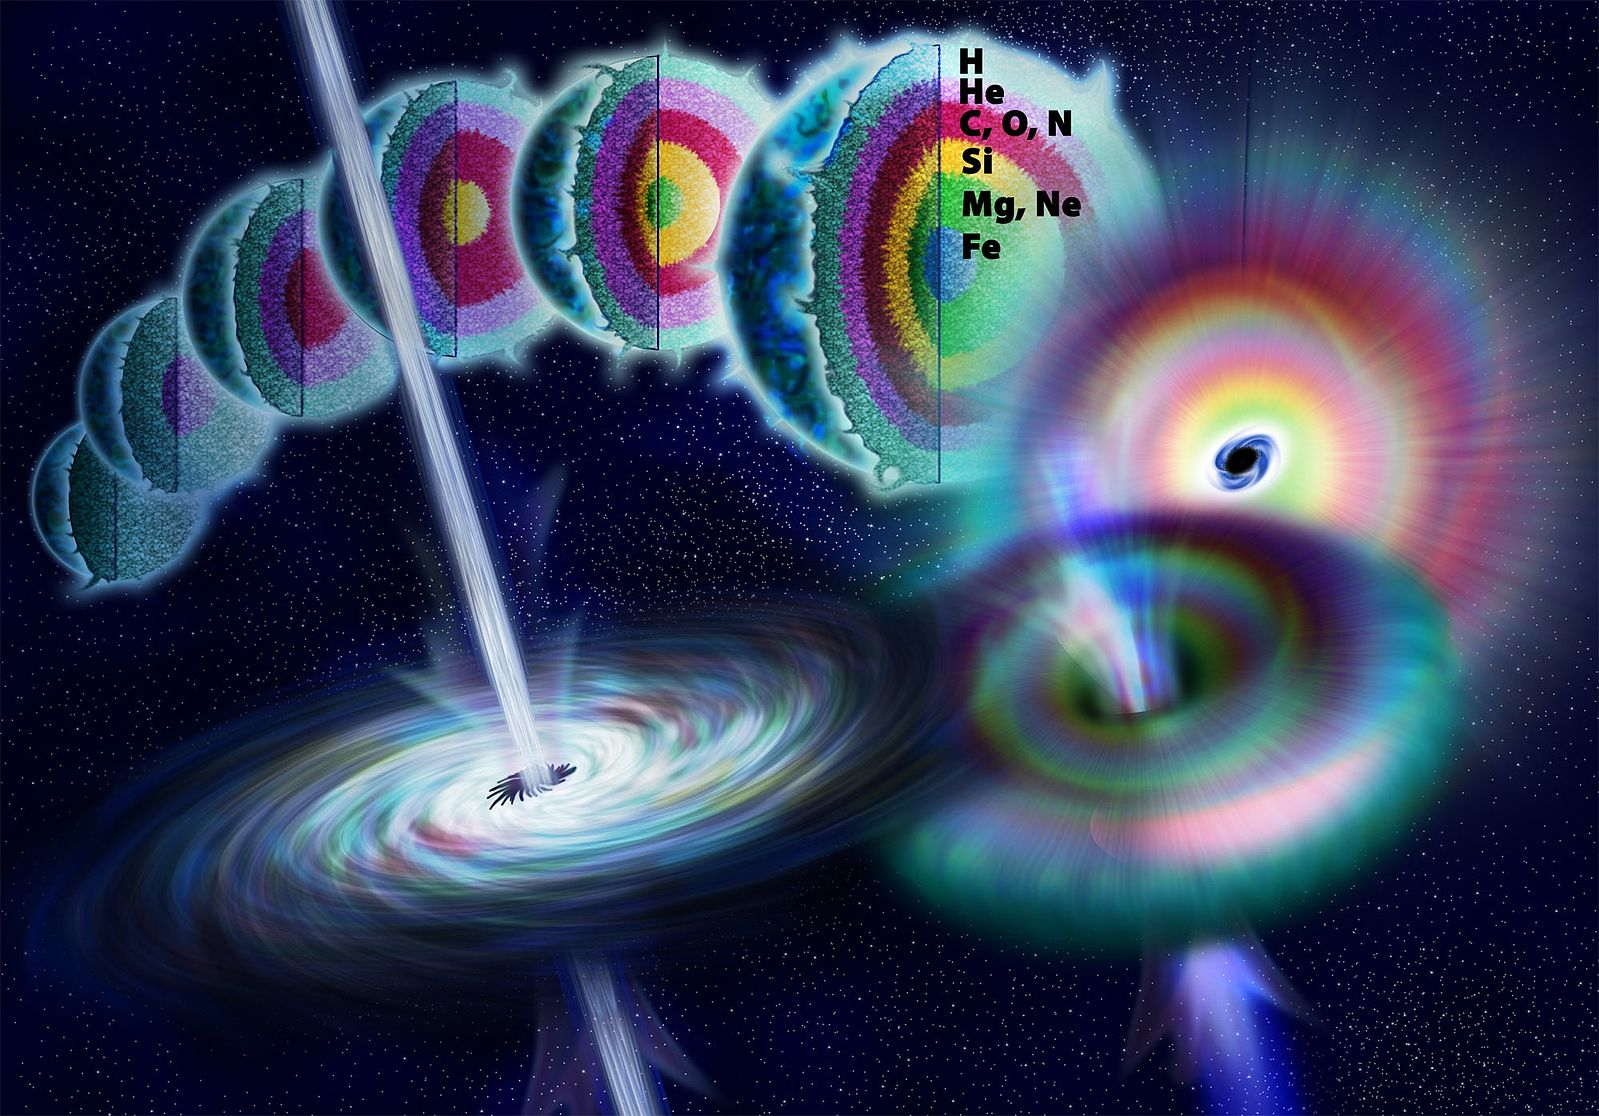
\includegraphics[width=130.0mm]{images/Gamma_ray_burst.jpg}
\caption{The life cycle of a massive star. When fusion stops the collapsing star releases energy in the form of jets observed as a gamma-ray burst}
\end{figure}

One of the most accepted theories describe GRBs as collisions of highly relativistic outflow of the accelerated jetted matter \cite{grb10}. For most of the observed GRBs the prompt $\gamma$-ray emission was followed by longer-lasting afterglow in soft X-ray, optical or radio waves \cite{grb11}. This is due to the propagation of a relativistic shockwave through the medium that surrounds the burst. Obsrvations proved that GRBs are at cosmological distances \cite{grb12}. The farthest GRB observed was at a distance of z=9.4. The avarge short GRBs lie at a distance of z=0.5. The long GRBs are even farther away, on avarage at z=2. The energy that is released is tremendous, about 10 erg. Long GRBs have been linked to the brightest regions of galaxies that contains the the most massive stars \cite{grb14}. %The relativistic outflow of LGRBs has a bulk Lorentz factor of $\Gamma\sim$300 [5]. The afterglow observations indicate that a geometrical beaming of the LGRBs radiation has an opening angle of $\sim$5 \cite{grb15}.

\begin{figure}[H]
\centering
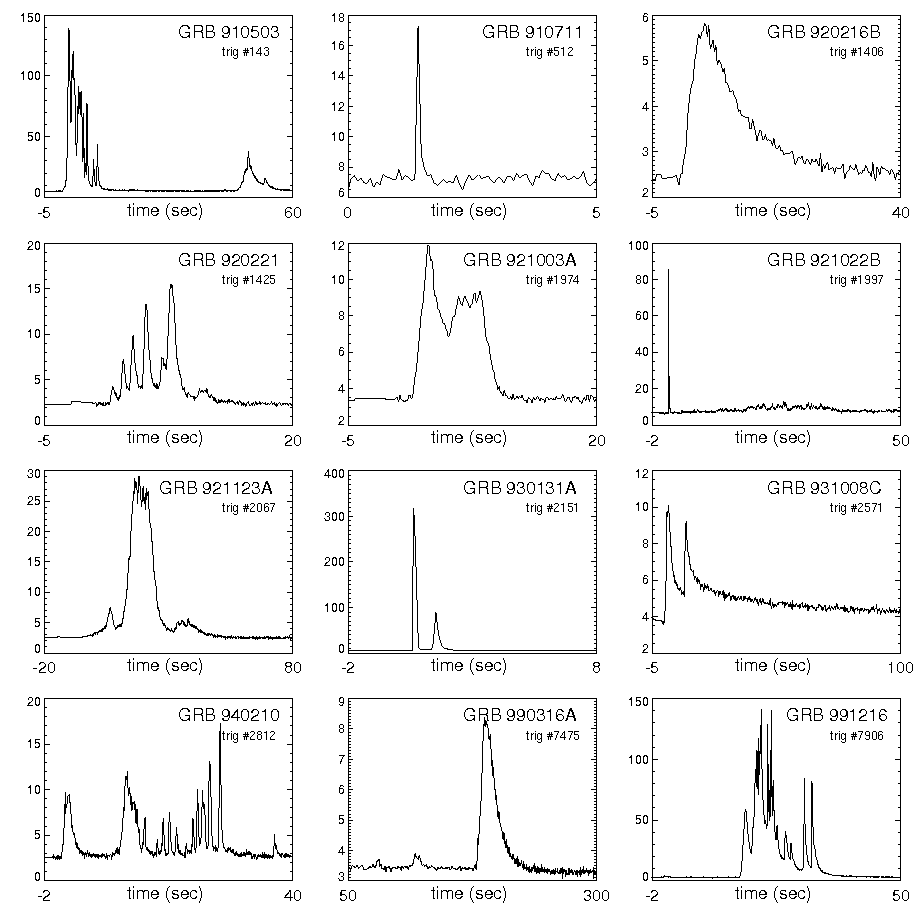
\includegraphics[width=130.0mm]{images/GRB_BATSE_12lightcurves.png}
\caption{The light curves of 12 gamma-ray bursts observed by BATSE. The diversity of the curves is extraordinary. Events with a length from millisecond to a second exist either with smooth or highly variable curves.}
\end{figure}

On the contrary, short GRBs are thought to originate in old populations. The theory that they originate from the merging of two neutron stars has been recently confirmed by detecting the gravitational waves of such an event. This was detected by the LIGO/Virgo collaboration in 2017 \cite{gravwave}. The electromagnetic counterpart of this gravitational wave event was detected as a short GRB by the Fermi/Gamma-ray Burst Monitor (GBM) and INTEGRAL instruments followed by the observation of the GRB’s afterglow and its host galaxy \cite{grb17}. Short GRBs emit electromagnetic radiation due to the radioactive decay of heavy r-process nuclei that are produced and ejected almost isotropically during the merger process \cite{grb18}.

\begin{figure}[H]
\centering
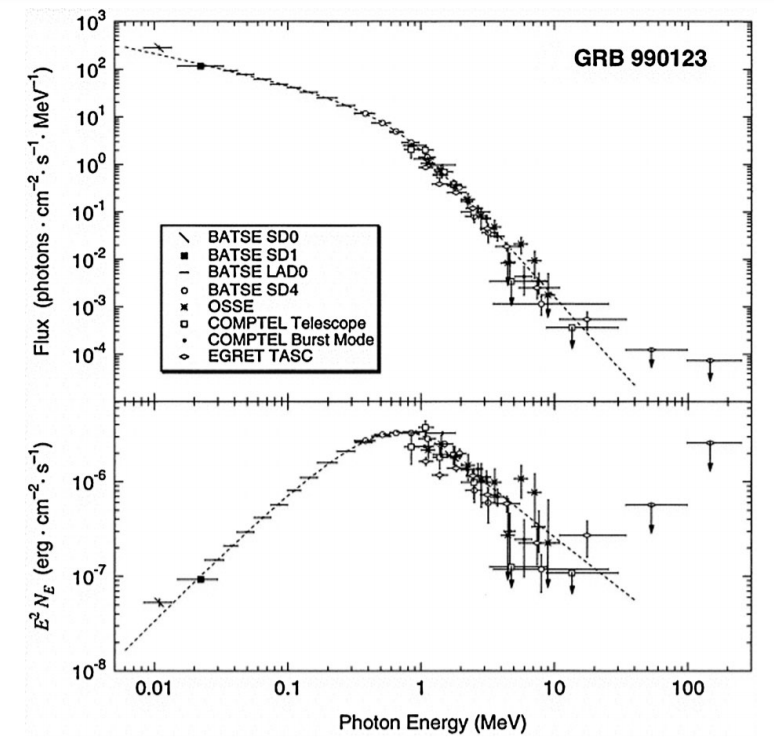
\includegraphics[width=130.0mm]{images/grb_spectra.png}
\caption{The band function of GRB 9900123 $\cite{grb_spectra}$}
\label{fig:grb_band}
\end{figure}

\subsection{Open questions on gamma-ray bursts}


Despite the fact that GRBs have been studied for more than fourty years a lot of questions are still not understood about their physics\cite{grb19}. In the following the main open questions are listed:

\begin{itemize}
\item{Classification: some of the observed light curves can not be classified into short and long GRBs, such as the ultra-long GRBs.}
\item{Central engine: in most cases it is thought that a black hole is formed after the merging of neutron stars and core collapse of massive starts. Although there are models that predict the birth of a magnetar. The most exotic theories predict the birth of a quark star that has never yet been observed.}
\item{Acceleration mechanism of the jets: How particles are accelerated to a velocity of Lorentz-factor of 300 in the shock waves is not yet understood.}
\item{GRB jet composition: there are two possible driving forces behind the acceleration of jet material. The first one is magnetic field dominated and the other one is dominated by baryons. As the acceleration of particles is not yet fully understood, it is not known whether protons can be accelerated to ultra-high energies. These could produce Ultra-High Energy Cosmic Rays.} 
\item{Radiation mechanism: there are several physical processes that create the $\gamma$-ray spectrum of GRBs, that is called  the "Band" function. The following three processes are though to be the main contributors to the spectrum: synchrotron radiation, synchrotron self-compton radiation and Compton up-scattering of thermal photons.}
\item{First stars: different population of stars on avarage have different masses. Models predit that population III stars end their life with a black hole that has a mass about ten times bigger than population I and II stars. The progenitors of GRBs can be classified into populations by their redshift \cite{grb20}.}

\end{itemize}

\subsection{Search for the electromagnetic counterparts of gravitational wave events}

Multi-messenger astronomy is based on the investigation of astronomical objects with disparate "messengers". It opened a possibility gather information in different ways to understand astrophysical objects. Until 2017 the three messenger were electromagnetic radiation, cosmic rays and neutrinos. 2017 opened a new era in multi-messenger astronomy as the electromagnetic counterpart of GW signal GW170817 was detected by the LIGO/Virgo collaboration. The source of this signal was the short GRB 170817A \cite{grb21}, a binary neutron star merger \cite{grb17}. 

This historical detection occured on August 17, 2017. The Fermi satellite detected the (short) GRB 170817A, approximately 1.7 s before to the detection of the GRB, LIGO-Virgo detector network observed a GW signal GW170817. The origin of this source was a neutron-neutron star merger. The source was localized  in a sky region of 28 deg$^{2}$ (with 90 \% confidence). 

After the detection of the GRB signal, several space and earth based observatories in a wide range of wavelengths started the investigation of the source. The discovery of a bright optical transient linked to the GRB was discovered in NGC 4993. Observatories involved in the investigation included Chandra X-ray Observatory \cite{grb23}, INTEGRAL \cite{grb22}, Swift and Nuclear Spectroscopic Telescope ARray (NuSTAR). A blue kilonova associated with this event was detected \cite{grb24}. It is important to emphasize that not only neutron-neutron star mergers but neutron star-black hole and black hole-black hole mergers can emit electromagnetic signal \cite{grb25}. Therefore all short GRBs can be investigated with multi-messenger astronomy in the future. As LIGO is constantly upgrading its detectors, gravitational waves will be detected more often. An even more sensitive gravitational wave detector is under building callled Kamioka Gravitational Wave Detector (KAGRA). First scientific measurements will be taken in the 2020s \cite{grb26}.

\subsection{Particle detectors in space}

Almost all types of detectors starting from semiconductor based detectors to gas-filled detectors have been used in space. In the case of search for GRBs the detection of x-rays is the most relevant. Several types of detectors can be used for detecting $\gamma$ photons\cite{grb30}, for example the semiconductor based  German Position Sensitive Proportional Counters (PSPC) of the ROSAT X-ray telescope. For our satellite the size of the detector is limited, therefore the best option was the usage of scintillators. Mostly used scintillators in space include inorganic crystal scintillators, for example NaI(Tl) or CsI(Tl), and plastic scintillators. CsI(Tl) was chosen as the detector of the Camelot CubeSat due to it's high light yield.

\subsection{Current missions observing gamma-ray bursts}

This subsection provides an overview of the existing missions that are aimed to detect GRBs. Field of view (FOV) an localization accuracy are chosen to compare them with the Camelot CubeSat. The proposed design of the Camelot satellite has the advantage of a large field of view and a high localization accuray. The main idea is that each CubeSat will detect GRBs at the same time. By measuring the time difference between the triggering of each satellite, the GRB soure can be triangularized. By using more satellites, the field of view will be the full-sky and localization accuracy increases.

The planed localization accuracy is more precise than any other existing GRB mission, that might reach $\sim$10'. While providing the highest lcoalization accuray, the field of view would also the be the highest, even larger than the field of view of the INTEGRAL/SPI-ACS and Fermi.

The size and mass of the Camelot CubeSat is less than 1\% of the Fermi telescope. Therefore from a fraction of the cost several satellites could be built and deployed in orbit. Having several satellites also provide a high redundance.

\begin{figure}[H]
\centering
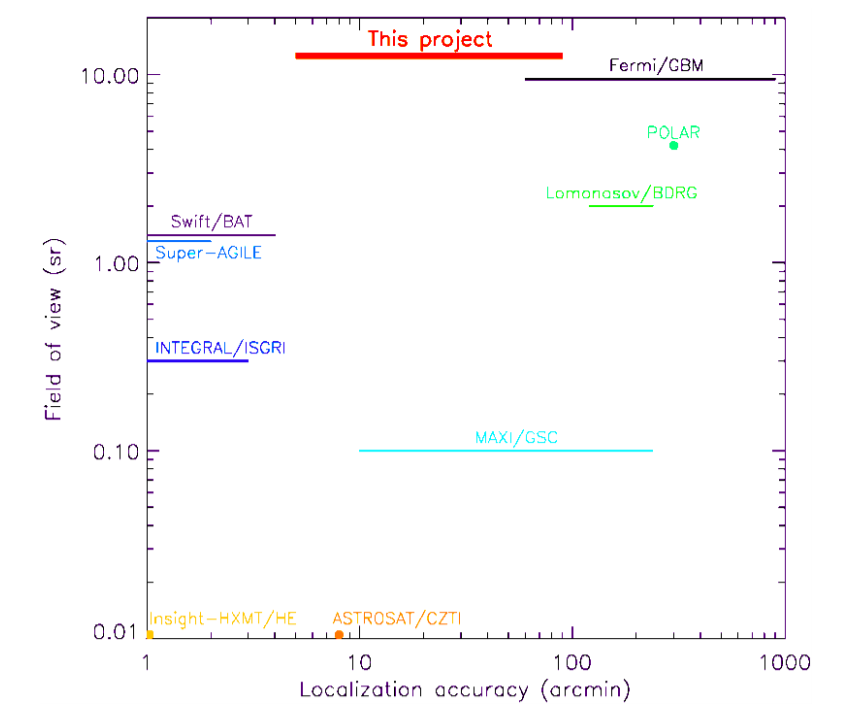
\includegraphics[width=130.0mm]{images/fovvsloc.png}
\caption{The field of view and localization accuracy of several missions including the Camelot CubeSat.}
\end{figure}

The following list includes the most relevant, currently ongoing missions looking for GRBs:

\begin{itemize}
\item Fermi 7 \cite{grb28} was launched in 2008 and its main instruments are Gamma-ray Burst Monitor and the Large Area Telescope (LAT). 
\item Neil Gehrels Swift Observatory (Swift) 8 \cite{grb31} was launched in 2005 and its main instruments are Burst Alert Telescope (BAT), X-ray Telescope (XRT), and UV/Optical Telescope (UVOT).
\item INTErnational Gamma-Ray Astrophysics Laboratory (INTEGRAL) 9 \cite{grb32} was launched in 2002. The most succesfull instruments on board include are the Anti-Coincidence Shield of the SPectrometer of INTEGRAL (SPI-ACS) and the Integral Soft Gamma-Ray Imager (ISGRI) detector layer of the "Imager on Board the Integral Satellite (IBIS)" detector.
\item Astro-Rivelatore Gamma a Immagini Leggero (AGILE) 11 \cite{grb34} was launched in 2007 and its Hard X-ray Imaging Detector (Super-AGILE) detected several GRBs.
\item CALorimetric Electron Telescope (CALET) 12 \cite{grb35} / Gamma-Ray Burst Monitor (CGBM), was launched in 2015 and it is placed on the International Space Station (ISS).
\item Monitor of All-sky X-ray Image (MAXI) 13 \cite{grb36}, started nominal observation in 2009. Its instrument Gas Slit Camera (GSC) detects GRBs. The instrument is placed on ISS.
\item Gamma-ray Burst Polarimeter POLAR 14 \cite{grb37}, was launched in 2016 and is dedicated to the measurement of GRB polarization.
\item Lomonosov 15 /BDRG \cite{grb38}, was launched in 2016. The BDRG instrument on board detected several GRBs.
\item The Hard X-ray Modulation Telescope (Insight-HXMT) 16 \cite{grb39}, was launched in 2017. It has on board the high energy X-ray telescope (HE), the medium energy X-ray telescope, and the low energy X-ray telescope.
\item ASTROSAT 17 \cite{grb40}, was launched in 2015 and its Cadmium Zinc Telluride Imager (CZTI) has already detected many GRBs.
\item Reuven Ramaty High Energy Solar Spectroscopic Imager (RHESSI) 18 \cite{grb41}, was launched in 2002. It is designed to study hard x-ray and gamma-ray emission from solar flares, however it is also efficient instrument to detect non-solar gamma-ray events like GRBs.
\end{itemize}


%\subsection{Currently operating GRB collection and alert networks}

%Our project can potentially contribute to some of the currently operating GRB collection and alertnetworks such as the following ones:
%The InterPlanetary Network (IPN) 27 \cite{grb42} which derives the positions of fast gamma-ray transients of all kinds by triangulation. Numerous spacecraft and instruments participate in the network at the Earth’s orbit as well as in the interplanetary space. It detects about 350/year.
%The Gamma-ray Coordinates Network (Transient Astronomy Network) (GCN/TAN) 28 provides information about GRBs in real-time to the world community. The network provides the real-time (and near real-time) distribution of GRB locations, images, spectra, and lightcurves detected by various spacecraft and the distribution of follow-up observation reports.
%The Global Relay of Observatories Watching Transients Happen (GROWTH) 29 is an international scientific collaborative project studying the astronomical transients.

%\subsection{Current GRB Follow-up observations}

%This cubesat project will provide high precision localization accuracy of GRBs allowing efficient follow-up observations by existing ground based observatories. There are several observatories world-wide to perform photometric or spectroscopic observations of GRB afterglows, for example:
%The Mobile Astronomical System of TElescope Robots (MASTER) 30 \cite{grb43} is a global network of robotic telescopes for very fast positioning and follow up of GRBs.
%The Burst Optical Observer and Transient Exploring System (BOOTES) network of robotic telescopes for follow up observations of GRBs. 31 \cite{grb44} is a world wide The Robotic Optical Transient Search Experiment (ROTSE) 32 [101] are telescopes which operate at sites around the world and follow GRBs.
%Pi of the Sky 33 [102] is a system of detectors designed for continuous observation of night sky looking for optical flashes of astrophysical origin, in particular for GRBs.
%Several other telescopes and observatories which provide measurements in optical, infra-red or radio bands are also, e.g.: Gamma-Ray Burst Optical/Near-Infrared Detector (GROND) 34 , the Palomar 60 inch telescope 35 , Rapid Eye Mount (REM) 36 , Livermore Optical Transient Imaging System (Super- LOTIS) 37 , Télescopes à Action Rapide pour les Objets Transitoires (TAROT) 38 , Gran Telescopio Canarias (GTC) 39 , ESO Very Large Telescope (VLT) 40 , Nordic Optical Telescope (NOT) 41 , Observatorio Astronómico Nacional on the Sierra de San Pedro Mártir 42 , Cerro Tololo Inter-American Observatory (CTIO) 43 , Telescopio Nazionale Galileo (TNG) 44 , Gao-Mei-Gu (GMG) station of Yunnan Observatories 45 , Observatorio de Sierra Nevada (OSN) 46 , United Kingdom Infrared Telescope (UKIRT) 47 , Very Large Array (VLA) 48 , Atacama Large Millimeter/Submillimeter Array (ALMA) 49 , James Clerk Maxwell Telescope 50 , Arcminute Microkelvin Imager which robotically triggers on Swift GRBs (AMI-GRB) 51 .

\subsection{The CAMELOT satellite}

There would most likely be four scintillators on the CAMELOT satellite. On two neighbouring sides of the satellite have two scintillators each. The scintillator will have a case either from aluminium or carbon fibre.

\begin{figure}[H]
\centering
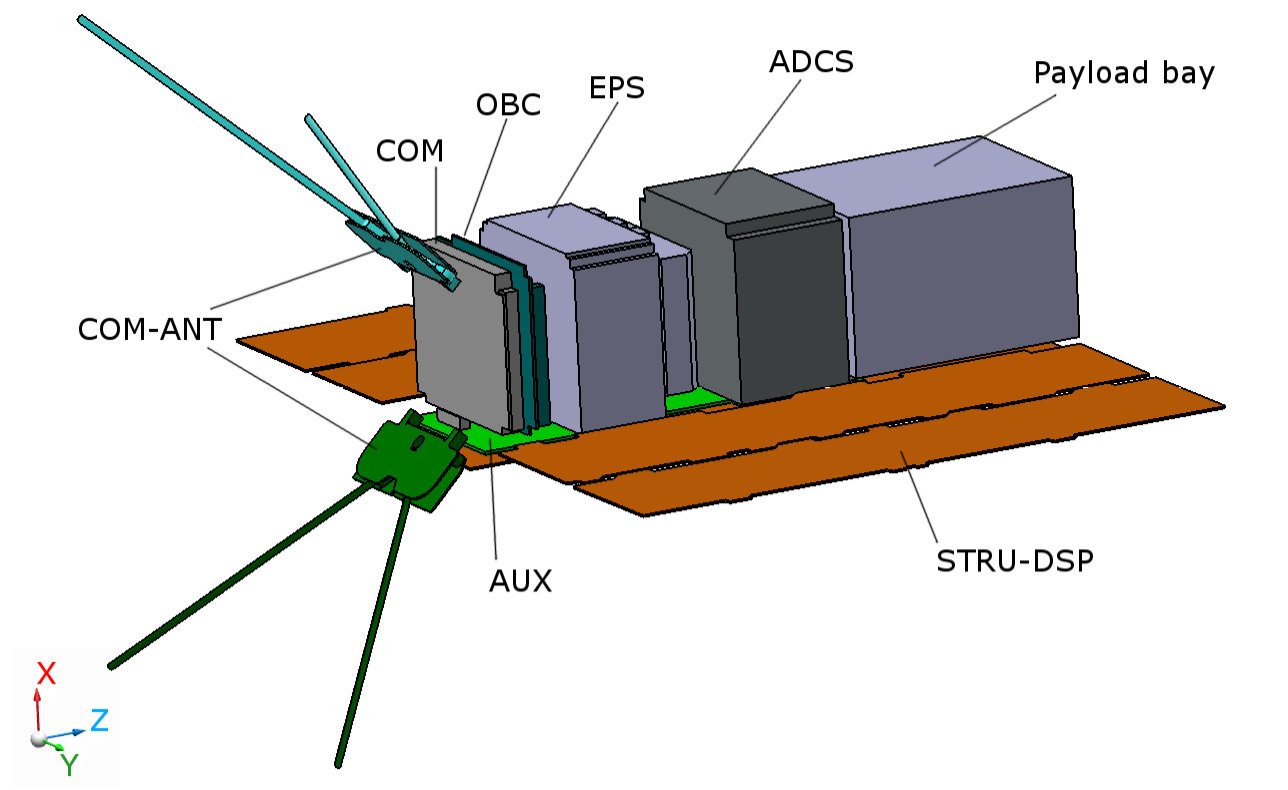
\includegraphics[width=130.0mm]{images/satellite_modules.png}
\caption{The modules of the satellite}
\end{figure}

The Camelot satellite will consist of the following modules:

\begin{itemize}
\item On-Board Computer [OBC] is responsible for control all the satellite’s sub-systems. OBC collects housekeeping and payload data and archives them in its internal storage.
\item Electrical Power System [EPS] is responsible for managing primary and secondary power sources and distributing power at appropriate voltage levels to on-board subsystems.
\item COM UHF Transceiver [COM] provides an RF communication link between the Ground Segment and the satellite. The COM codes the received messages from the OBC and transmits to the Ground Segment. Furthermore, the COM decodes the received RF messages from the Ground Segment and transmits to the OBC.
\item Attitude Determination and Control System [ADCS] determines and controls the satellite attitude.
\item Auxiliary Electronics [AUX] subsystems control the deploying mechanisms and monitor the
solar arrays. The Aux subsystem also contains the rigid backplane of the satellite; therefore, it also connects the subsystems.
\item Structure [STRU]
\item Ground Support Equipment [EGSE]
\end{itemize}

\subsection{The detection of GRBs}

The current detector design is a combination of CsI scintillators reaodout by the Multi Pixel Photon Counter (MPPC), which is a kind of the Silicon Photomultiplier device. The advantage of this system is a high light output with compact readout area. For the localization of GRB, photon statistics is one of important issue. Therefore, we need as much light yield as possible. Also, since the detector mounting area for the 3U cubesat standard is limited to be $\sim$300x75x5 mm$^{3}$ as described in the beginning of this section, a compact readout device is required. Currently, we are evaluating the detector performance using a sample of detector system consist of CsI(Tl) scintillator with a dimension of 150x75x5 mm$^{2}$ readout by Hamamatsu MPPC (latest model: S13360-6050CS with an effective area of 6x6 mm$^{2}$). \ref{fig:schem} shows a schematic picture of the location of one side of the detector and actual setup of performance evaluation test.

\begin{figure}[H]
\centering
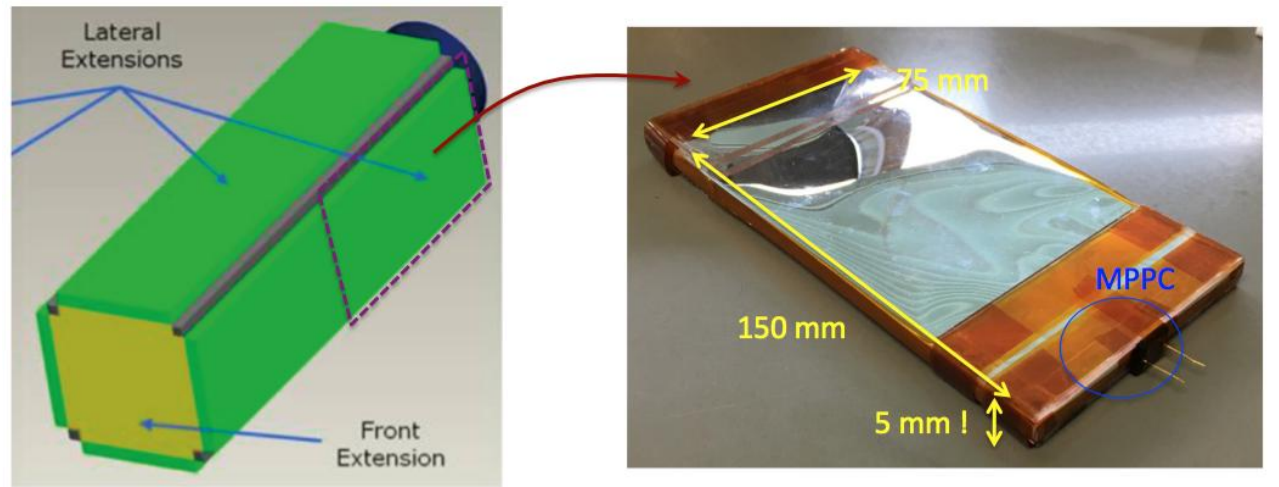
\includegraphics[width=130.0mm]{images/scint_on_sate.png}
\caption{Side extensions including of the CAMELOT satellite (left) where scintillators are placed and and a wrapped scintillator with the MPPC read out (right)}
\end{figure}

It is challenging to readout the scintillation photons for such geometrically large and thin crystal with small readout area because the produced scintillation photons would be suffered by the multiple scattering inside the crystal before reaching the readout area of the MPPC. This would degrade the final light yield and affect to the performance of the energy resolution and lower energy threshold. In order to overcome this problem, we are planning to apply a multi-channel coincidence readout technique. A multi-channel readout increases the readout area and final light yield, simply and improvement of the uniformity of the light yield with respect to the incident gamma-ray position would be expected. However, increasing of the readout channel also increase the leakage current, which would be proportional to the readout area. The coincidence readout technique would be expected to suppress the effect of the increasing of the leakage current in the resultant spectrum. 

\begin{figure}[H]
\centering
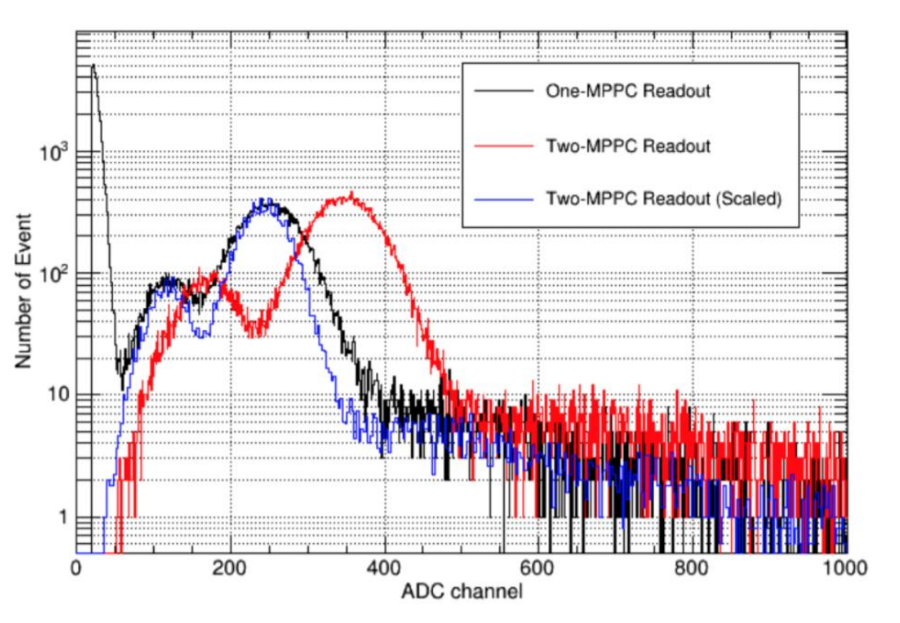
\includegraphics[width=130.0mm]{images/histo_for_det.png}
\label{fig:spectras_meas}
\caption{Energy spectra obtained by collecting the signal of 1 million $\gamma$ with the one channel and the two channel read out}
\end{figure}

Figure 23 shows the latest result of the study of this technique by irradiating 241Am radioisotope. Black and red data show the result by the single channel and 2-channel coincidence readout the single channel readout, respectively. As one can see obviously, the final light yield corresponding to the 59.5 keV gamma-ray photo absorption peak increases by almost 50 \% for the 2-channel readout. By scaling  the 2-channel readout result to the single channel readout for the 59.5 keV peak as shown by the blue curve, we found that the energy resolution improved thanks to the improvement of the uniformity of the position dependence of the light yield. Finally, we confirmed that the lower energy threshold for both readout technique achieved to be about 10 keV. Further improvement of the uniformity and/or lower energy threshold could be possible by optimizing the install location of the MPPC device.

\subsection{The Geant4 platform}

Geant4 \cite{geant1, geant2, geant3} (for GEometry ANd Tracking) is a platform for "the simulation of the passage of particles through matter," using Monte Carlo methods. It is the successor of the GEANT series of software toolkits developed by CERN, and the first to use object oriented programming (in C++). Its development, maintenance and user support are taken care by the international Geant4 Collaboration. Application areas include high energy physics and nuclear experiments, medical, accelerator and space physics studies. The software is used by a number of research projects around the world.

The Geant4 software and source code is freely available from the project web site; until version 8.1 (released June 30, 2006), no specific software license for its use existed; Geant4 is now provided under the Geant4 Software License.

\begin{figure}[H]
\centering
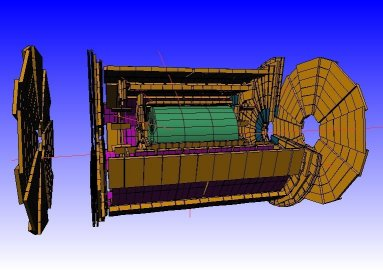
\includegraphics[width=130.0mm]{images/AtlasHalf.jpg}
\caption{The Geant4 simulation of the whole ATLAS experiment}
\end{figure}

Geant4 includes facilities for handling geometry, tracking, detector response, run management, visualization and user interface. For many physics simulations, this means less time needs to be spent on the low level details, and researchers can start immediately on the more important aspects of the simulation.

Following is a summary of each of the facilities listed above:

Geometry is an analysis of the physical layout of the experiment, including detectors, absorbers, etc., and considering how this layout will affect the path of particles in the experiment.
Tracking is simulating the passage of a particle through matter. This involves considering possible interactions and decay processes.
Detector response is recording when a particle passes through the volume of a detector, and approximating how a real detector would respond.
Run management is recording the details of each run (a set of events), as well as setting up the experiment in different configurations between runs.
Geant4 offers a number of options for visualization, including OpenGL, and a familiar user interface, based on Tcsh.
Geant4 can also perform basic histogramming; it requires external analysis tools or software that implements the AIDA framework for exploiting advanced histogramming features.

Since release 10.0, Geant4 implements multithreading, making use of thread-local storage to allow for efficient generation of simulated events in parallel.

Because of its general purpose nature, Geant4 is well suited for development of computational tools for analysing interactions of particle with matter in many areas. These include:

Space applications where it is used to study interactions between the natural space radiation environment and space hardware or astronauts; Medical applications where interactions of radiations used for treatment are simulated. Radiation effects in microelectronics where ionizing effects on semiconductor devices are modeled.

\subsection{The experimental setup}


We are designing a fleet of nanosatellites to perform accurate position determinations
of short-duration gamma-ray bursts by measuring arrival time differences.
To achieve sufficient photon statistics to measure the arrival times
precisely under the severe limitations of size, mass, and power consumption,
we propose the use of a large-area CsI scintillator that has high light output
and the use of a small-sized multipixel photon counter (MPPC) that has low
power consumption. We plan to use one of the latest-model MPPCs provided
by Hamamatsu Photonics, which has an active area of 6  6 mm2. We have compared the performance of two scintillators of different sizes (150  75  5 mm3 and 100  75  5 mm3); the bigger one is the maximum size that can be mounted on a three-unit satellite, according to CubeSat standards.
We have found that the two scintillators have similar light yields and each has an energy threshold of $\sim$10 keV at 25C. We have also examined the position dependence of the light yield by using radiation from 241Am (59.5 keV) source, and have confirmed that uniformity was improved by using two MPPCs for signal readout. 

\begin{figure}[H]
\centering
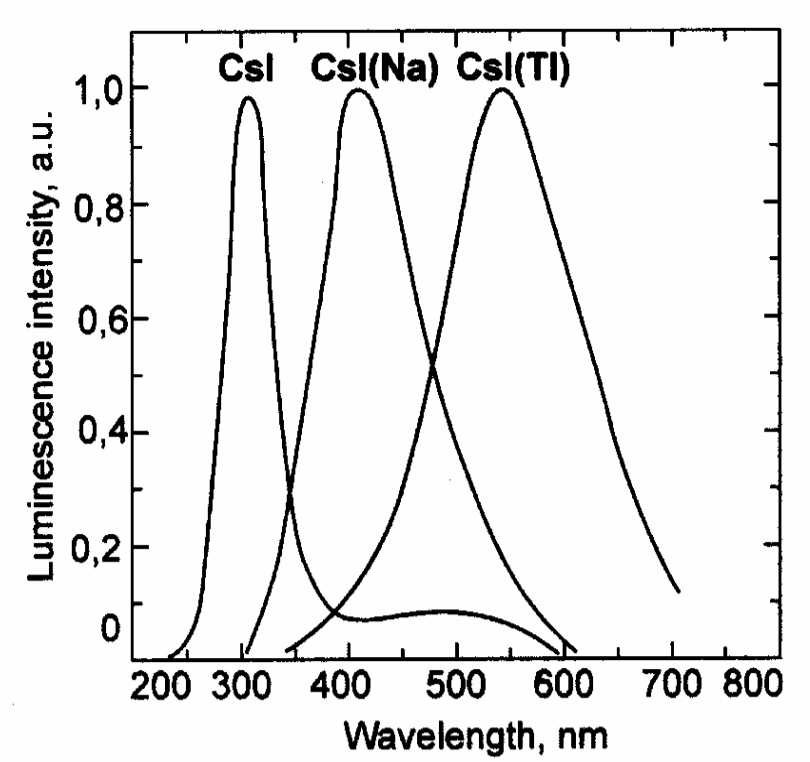
\includegraphics[width=130.0mm]{images/spectracsitl.png}
\caption{The emitted scintillation light spectra of three types of scintillators. In our experiment CsI(Tl) was used}
\end{figure}



\begin{figure}[H]
\centering
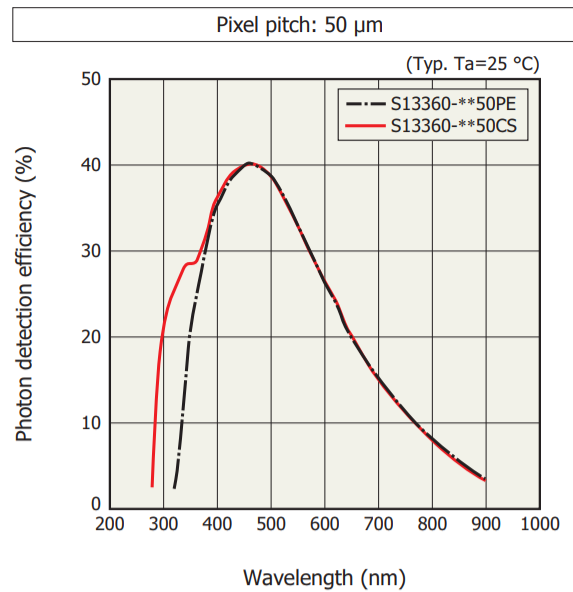
\includegraphics[width=130.0mm]{images/qe.png}
\caption{The photon detection efficiency $\cite{qe}$ of the MPPCs used for the readout of the scintillators. This data was included in the simulation.}
\end{figure}


\begin{figure}[H]
\centering
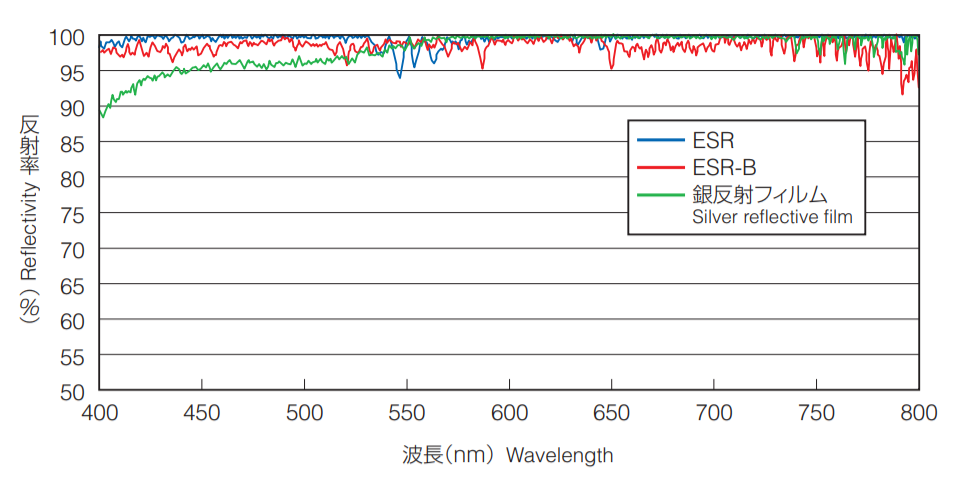
\includegraphics[width=130.0mm]{images/reflectivity.png}
\caption{The reflectivity $\cite{scinti}$ of the ESR tape that was used to wrap the scintillator in order to increase the light yield. This data was included in the simulation.}
\end{figure}


HAMAMATSU S13360-6050CS

ESR foil

QE \cite{qe} of the MPPC


datasheet of QE:
%http://www.hamamatsu.com/resources/pdf/ssd/s13360_series_kapd1052e.pdf

esr \cite{esr} foil:
Please check "ESR from 3M" company. e.g.,
%http://multimedia.3m.com/mws/media/466120O/esr.pdf



\subsection{Simulation}

In order to understand how the $\gamma$ photons -- that the CubeSat is meant to detect -- interact with the matter of the satellite simulations are needed. In a simulation it is also possible to determine the optimal geometry that would lead to the best GRB detection. 

The Geometry... XXX TRacking (Geant4) 


The cross section for photoeffect is far the largest by far for low energy gamma photons.
The ionized nuclei and the secondary electrons generates scintillation.

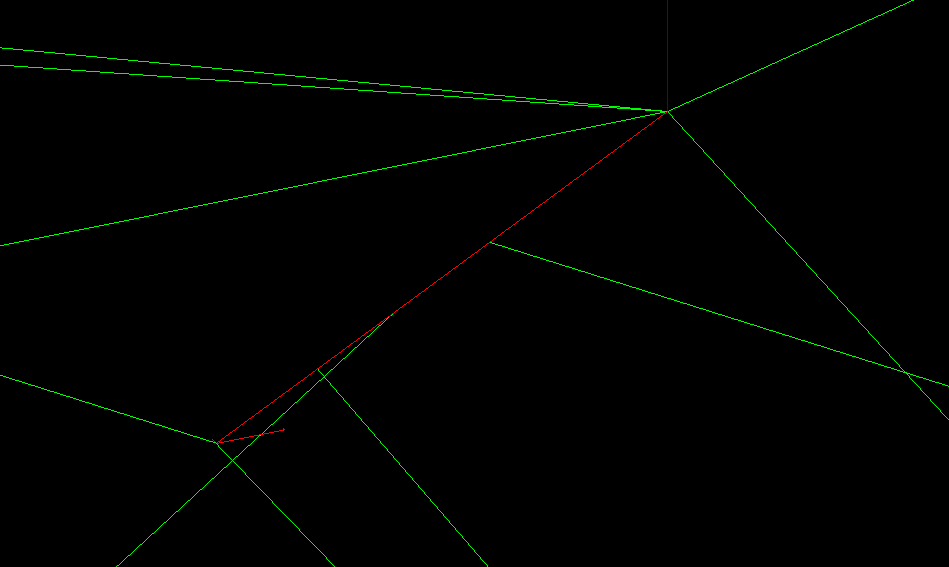
\includegraphics[width=130.0mm]{images/secondary.png}


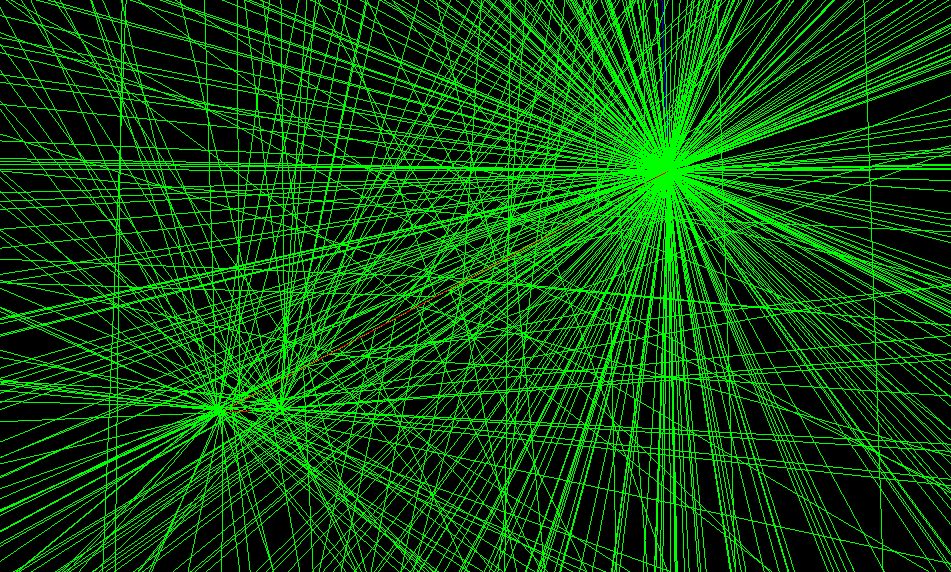
\includegraphics[width=130.0mm]{images/secondary2.png}

Also the nuclei that is ionized by the gamma produces photons.

\section{Setup}

We obtained energy spectra by using two radioisotopes (109Cd and 241Am) to evaluate the performance of our CsI scintillator + MPPC system. We placed a CsI scintillator and an MPPC in an aluminum case (2 mm thick) installed in the thermostatically controlled chamber (ESPEC LU-113). We set the operating temperature to 25C. We first tested a one-MPPC readout by using a commercial charge-sensitive preamplifier (CLEAR-PULSE 5028), a shaping amplifier (EG\&G ORTEC 571), and an ADC (AMPTEC MCA800A). We set the shaping time to 1 $\mu$s. We then tested a two-MPPC readout by using an 3 FADC Board (SHIMAFUJI Electric) originally developed for an astrophysical polarimetry mission PoGO+ [9] in order to read and sum the signals of coincident events; the shaping time for this test was set at 2.2 $\mu$s.
Figure 1 shows the setup of the experiment. We installed two lead sheets (identical in size to the scintillator) to collimate signals from the radioisotopes(3.3). We tested two CsI scintillators obtained from Amcrys with different sizes (150  75  5 mm3 and 100  75  5 mm3). Each was covered with one layer of ESR as a reflector. We used one of the latest-model MPPCs by Hamamatsu Photonics, namely, S13360-6050CS, which has an active area of 6  6 mm2 [10]. We attached an MPPC to the center of the narrower side plane of the scintillator (with an area of 75  5 mm3) for the one-MPPC readout. For the two-MPPC readout, we attached the MPPCs 18.75 mm from the edge of the plane. The breakdown voltages of the two-MPPCs are almost the same–50.82 and 50.87 V–at 25 C. We used a KEITHLEY 2400 to supply the operational voltage of 53.4 V. In analyzing of the obtained data, we evaluated four items:
the light yields of the two scintillators, the energy thresholds, the
uniformity of the light yield, and the energy resolution.

\begin{figure}[htbp]
 \centering % \begin{center}/\end{center} takes some additional vertical space
 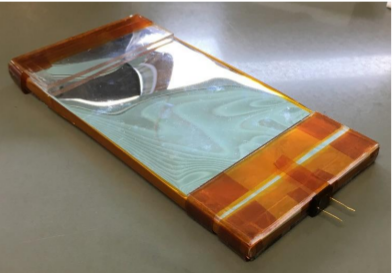
\includegraphics[width=.4\textwidth,origin=c,angle=0]{images/1channelsetup.png}
 \qquad
 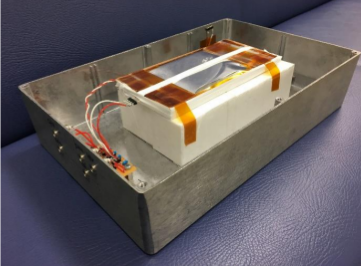
\includegraphics[width=.4\textwidth,origin=c,angle=0]{images/1channelsetupbox.png} 
 % "\includegraphics" from the "graphicx" permits to crop (trim+clip)
 % and rotate (angle) and image (and much more)
 \caption{\label{fig:i} The scintillator on the left and the cage holding the setup on the right}
 \end{figure}


\begin{figure}
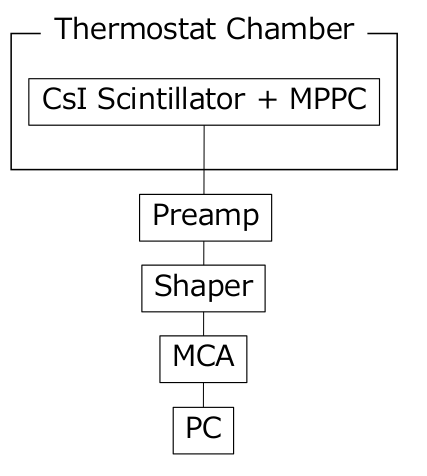
\includegraphics[width=130.0mm]{images/1channelelectronics.png}
\caption{The schematic design of the readout of the MPPC for the 1 channel configuration}
\label{fig:el1ch}
\end{figure}



\begin{figure}
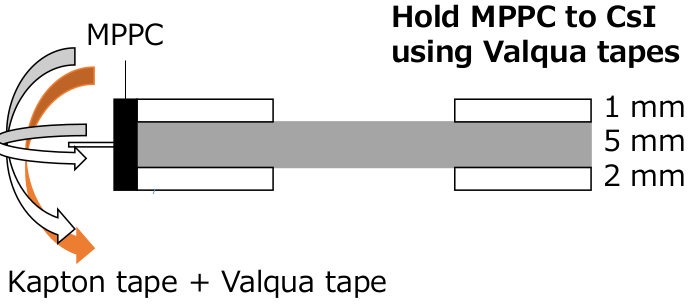
\includegraphics[width=130.0mm]{images/tap1channel.png}
\caption{\label{fig:1channeltape} The MPPC is fixed to the scintillator with valqua tape}
\end{figure}



Size of the scintillator is, the aluminium housing thickness is, the size of the SiPM is...

Parameters of the CsI(Tl) scintillator REF



\begin{table}[h!]
\begin{center}
\begin{tabular}{ |c|c|c|c|c|c|c|c|c|} 
 \hline
 Energy [eV] & 3.54 & 3.10 & 2.76*eV & 2.48*eV & 2.36*eV & 2.25*eV & 2.07*eV & 1.91*eV\\\hline
 Relative emittance & 0.02 & 0.1 & 0.3 & 0.6 & 0.9 & 1.0 & 0.7 & 0.4 \\\hline
 Refractive index & 1.59 & 1.57 & 1.54 & 1.54 & 1.54 & 1.54 & 1.54 & 1.54 \\\hline
 Absorption lengh [cm] & 50 & 50 & 50 & 50 & 50 & 50 & 50 & 50  \\\hline
 

 \hline
\end{tabular}
\end{center}
\caption{The mass ratio of materials that are used for the satellite}
\end{table}



%  CsI_mt->AddConstProperty("RESOLUTIONSCALE",1.0);
%  CsI_mt->AddConstProperty("SLOWTIMECONSTANT",200.*ns);
%  CsI_mt->AddConstProperty("YIELDRATIO",1.0);
  
% G4double glass_RIND[lxenum]={1.49,1.49,1.49};
%  G4double glass_AbsLength[lxenum]={420.*cm,420.*cm,420.*cm};  
%  G4double reflectivity[num] = {0.995, 0.995};
%G4double photocath_EFF[num]={1.,1.}; //Enables 'detection' of photons
%  G4double photocath_ReR[num]={1.92,1.92};
%  G4double photocath_ImR[num]={1.69,1.69};

\begin{itemize}
\item Scintillation yield (Number of photons produced by given keV depleted in the scintillator): 540 1/keV
\item The time constant of the scintillation photon creation: 200 ns (exponential decay)
\end{itemize}

Optical parameters of the materials and surfaces:
\begin{itemize}
\item Refractive indices of all relevant materials
\item Reflection
\item The detection efficiency of the SiPM detectors
\end{itemize}

\subsection{1 channel setup}

\begin{figure}
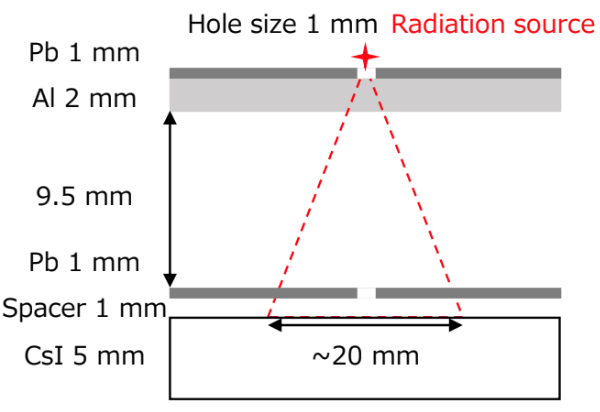
\includegraphics[width=150.0mm]{images/irradiation.png}
\caption{The $^{241}$Am $gamma$ source was placed in a collimator system as can be seen on the image}
\end{figure}

The $\gamma$ source that was used to test the experimental setup was choosen to be an $^{241}Am$. The reason for this is that the peak of energy spectrum of the $\gamma$ photons from GRBs is at 50 keV which is very close to the peak of the $^{241}Am$ that is 59.5 keV. The activity of the source at the time of the experiment was 471 kBq. The source was collimated to a beam that hit the surface of the scintillator on a circle with a radius of 10 mm. The distance of the source from the scintillator was 13.5 mm. Therefore the solid angle of the part of the whole sphere where $\gamma$s could be detected was 
$$\Theta = 2 \pi (1-cos(\theta)) = 1.234 sr$$

 Therefore the number of $\gamma$s that hit the scintillator, the Al and Pb sheets above it was:
$$A = \frac{1.234}{4 \pi} \cdot 471 kBq = 46.25 kBq$$

\pagebreak

\subsection{2 channel read out setup}

\begin{figure}[h!]
\centering
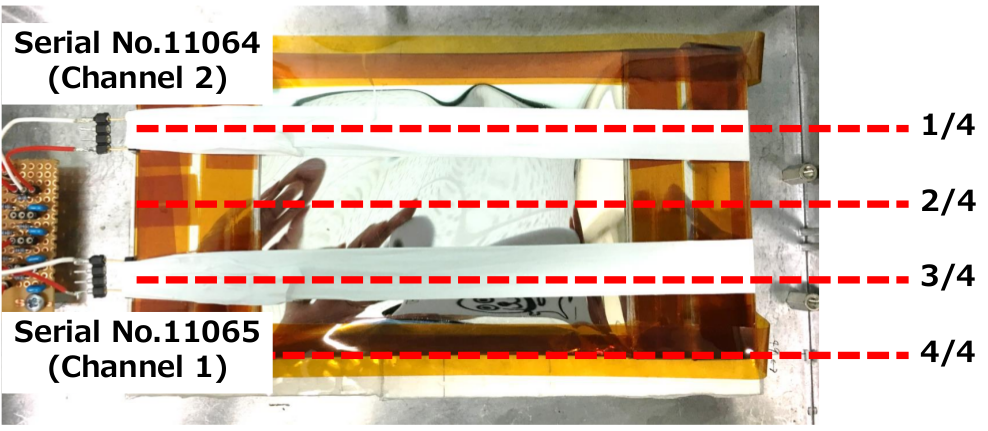
\includegraphics[width=130.0mm]{images/2channelsetup.png}[H!]
\caption{The MPPCs for the 2 channel readout are positioned symmetrically from the center of the scintillator}
\end{figure}

\begin{figure}[h!]
\centering
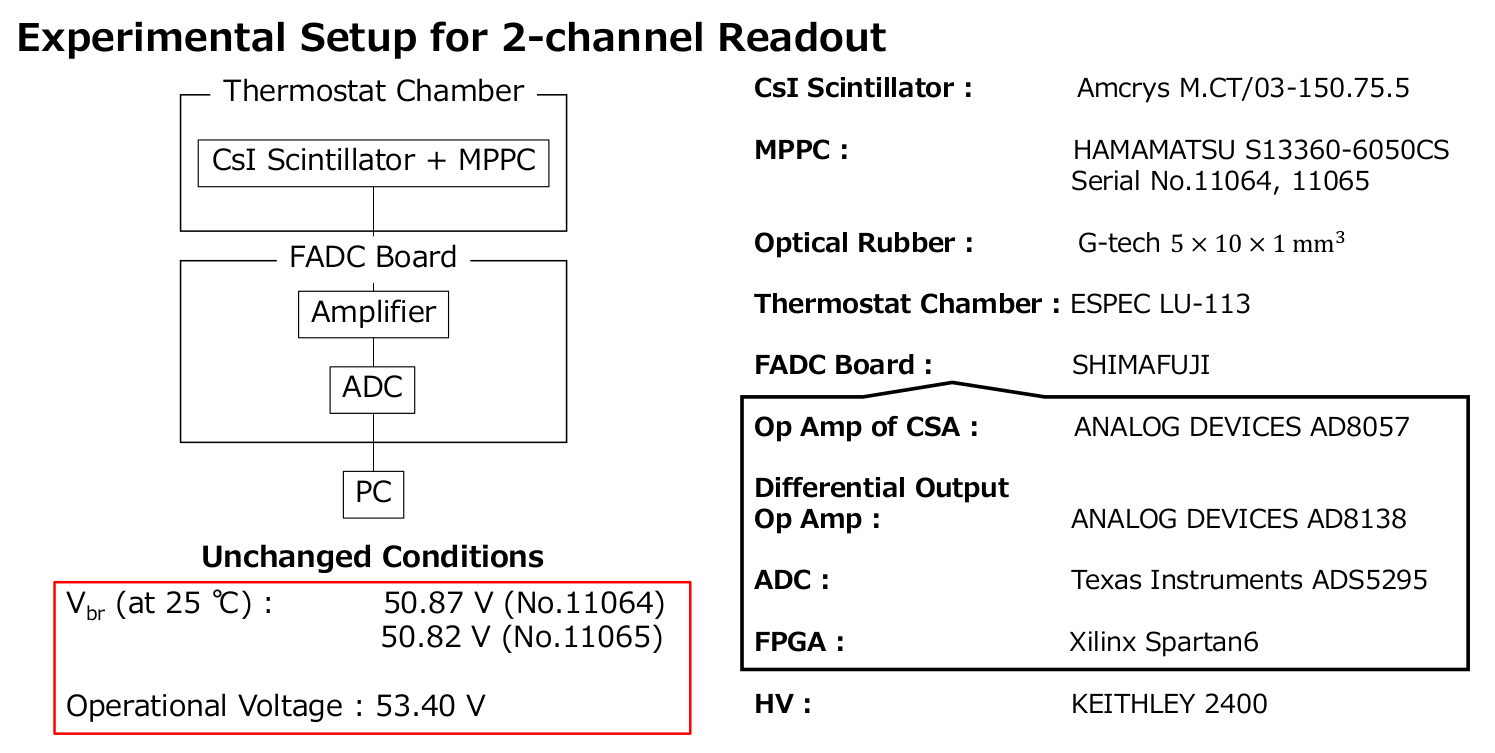
\includegraphics[width=130.0mm]{images/2channelelectronics.png}
\caption{The schematic design of the readout electronics of the 2 channel setup}
\end{figure}

\begin{figure}[h!]
\centering
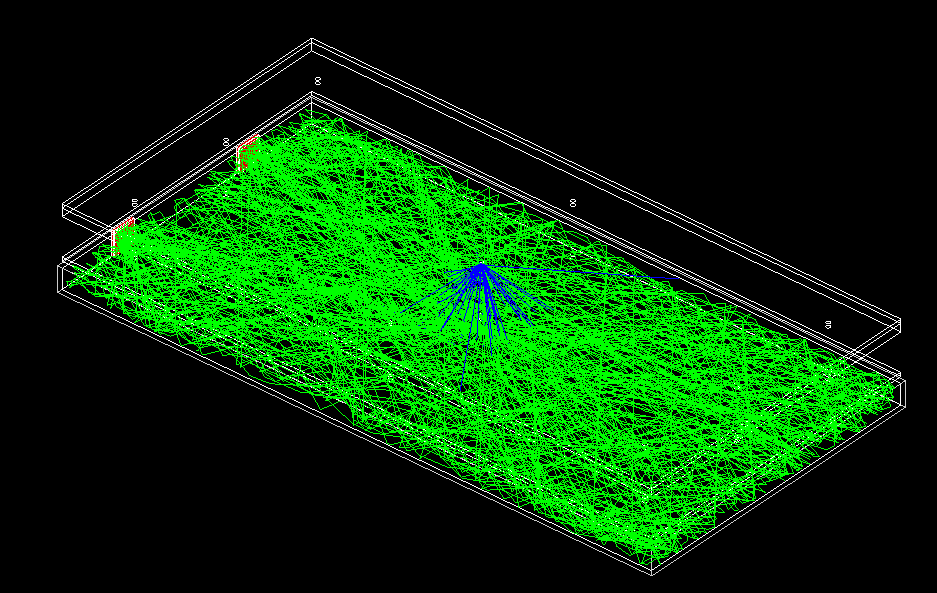
\includegraphics[width=160.0mm]{images/2channel.png}
\caption{Simulation of 100 $\gamma$s emitted from the source. The blue lines represent the track of the $\gamma$s and the green lines represent the track of the optical photons created by scintillation. Only the photons that were detected are drawn.}
\label{fig:sim_setup}
\end{figure}

\pagebreak

\subsection{The satellite}

The direction of GRBs is isotropic in the sky as they are extragalactic objects. As the positioning of the scintillators is not decided yet it is important to understand which configuration would be the best for detecting as many GRBs as possible. Therefore it is vital to understand how the material of the satellite itself absorbs $\gamma$s. The satellite consists of several modules with specific shapes and material contents. Therefore building up the whole geometry and material composition was not possible in Geant4, thus the model of the satellite had to be  imported into Geant4.

\begin{figure}[h!]
 \centering % \begin{center}/\end{center} takes some additional vertical space
 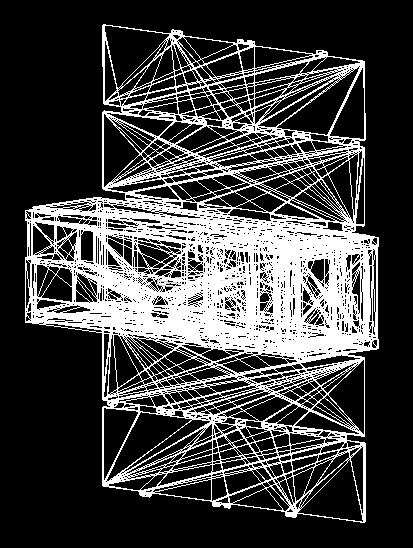
\includegraphics[width=.3\textwidth,origin=c,angle=0]{images/satellite.png}
 \qquad
 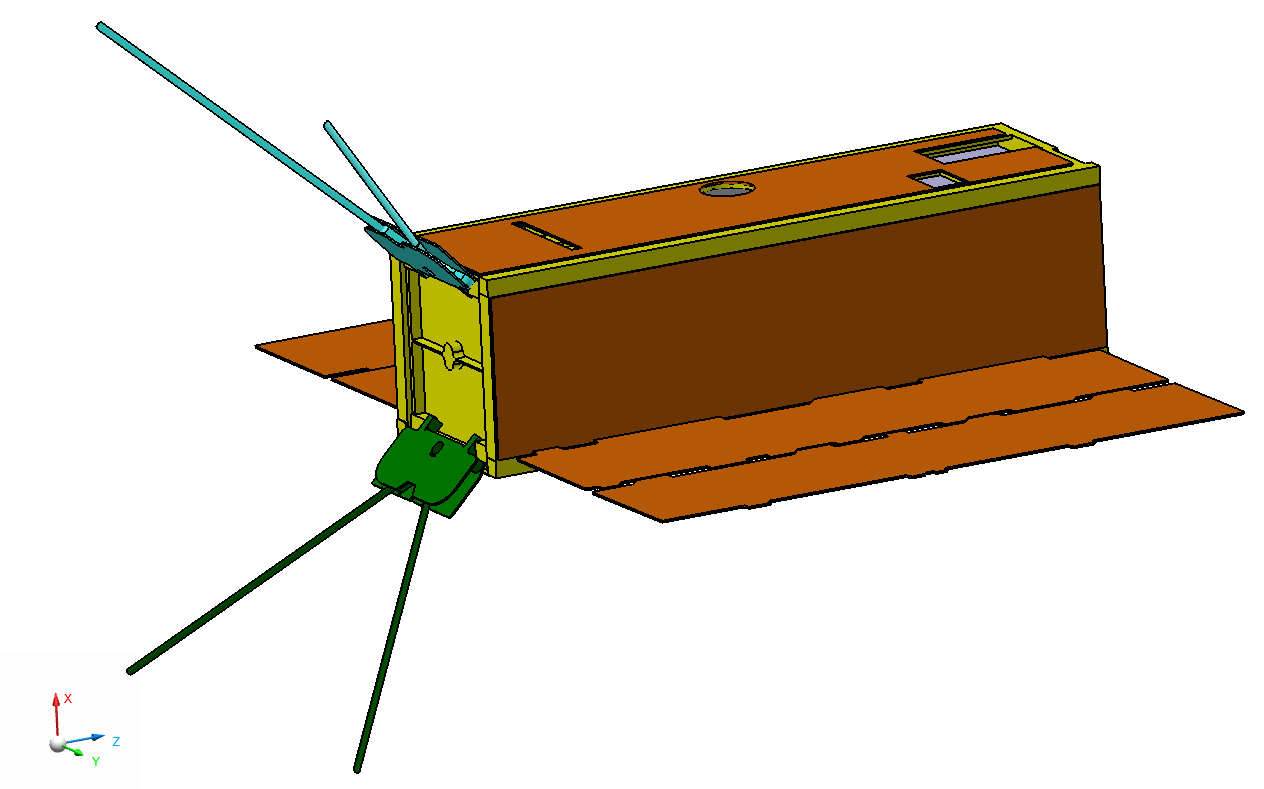
\includegraphics[width=.5\textwidth,origin=c,angle=90]{images/cad_sat.png} 
 % "\includegraphics" from the "graphicx" permits to crop (trim+clip)
 % and rotate (angle) and image (and much more)
 \caption{\label{fig:i} The CAD model of the satellite (on the right) and the view of the imported model in Geant (on the left)}
 \end{figure}

Importing predefined CAD models into GEANT4 is not always possible or requires intermediate file format conversion to Geometry Description Markup Language (GDML) using commercial or third party software. CADMesh \cite{cadmesh} is a direct CAD model import interface for GEANT4 leveraging ASSIMP \cite{assimp} for reading the CAD files. In this work the CAD model of the satellite was exported to STL files. These files were imported by the CADMesh software to Geant4. The tesselation was done by the TETGEN \cite{tetgen} software.

\begin{figure}[h!]
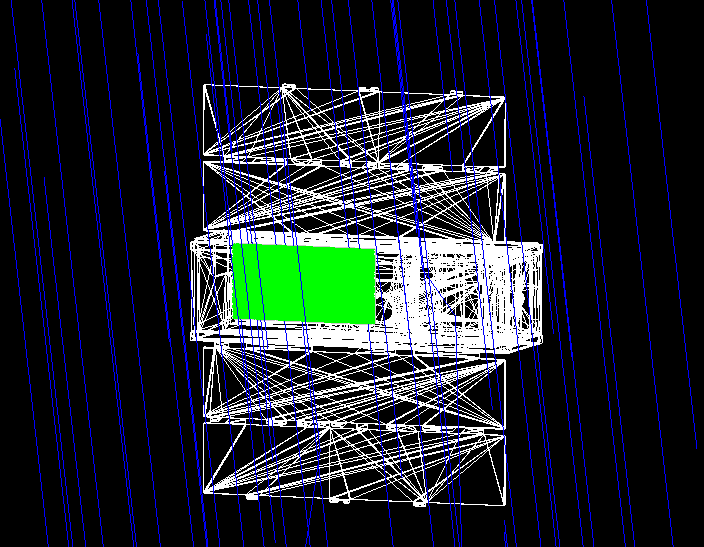
\includegraphics[width=150.0mm]{images/satellite_rad.png}
\caption{The satellite radiated by a pencil beam of 10.000 $\gamma$ particles. The scattered $\gamma$s induce signal in the scintillator}
\end{figure}

\begin{table}[h!]
\begin{center}
\begin{tabular}{ |c|c|c|c|} 
 \hline
 Name of module & mass [g] & Type of material & Mass ratio [\%]\\\hline
 ADCS &	710	& Aluminum 6061-T6 &	50\\
			& & Copper Electric	& 25 \\
			& &  Glass Borosilicate 	& 25\\\hline
COM	& 	90	& 	Stainless Steel 	& 2\\
			& 	& Brass Generic		& 25\\
			& 	& Aluminum 7075-T73		& 40\\
			& 	& FR4 Glass-Epoxy sheet	& 	33\\\hline
EPS	& 	750	& 	FR4 Glass-Epoxy sheet		& 25\\
			& 	& Aluminum 6061-T6		& 75\\\hline
OBC	&	50		& FR4 Glass-Epoxy sheet	& 	100\\\hline
STRU	& 	980		& Aluminum 6061-T6	& 	100\\\hline
SP	& 	570		& Solar Panel	& 	100\\\hline
Payload	& 	1100	& 	As you wish	& 	100\\
 \hline
\end{tabular}
\end{center}
\caption{The mass ratio of materials that are used for the satellite}
\end{table}

\begin{table}[h!]
\begin{center}
\begin{tabular}{ |c|c|c|c|c|c|c|c|c|c|c|c|c|} 
 \hline
%Material name & El. 1	& El. 1 m.r. & El. 2 & El. 2 m.r. &El.3	& El. 3 m.r. &El. 4	& El. 4 m.r. &El.	5& El. 5 m.r. &El.	6& El. 6 m.r. \\\hline
Material name & &&&&&&&&&&& \\\hline

Aluminum 6061-T6 &	Al & 96.90 &	Mg &	1.20 &	Si &	0.80 &	Fe &	0.70 &	Cu &	0.40 & &\\\hline		
Aluminum 7075-T73 &	Al &	88.60 &	Zn &	6.10 &	Mg &	2.90 &	Cu &	2.00 &	Si &	0.40 & &\\\hline		
%Stainless Steel A2-70  AISI 304 (EN 1.4301) &	Fe &	66.50 &	Cr &	20.00 &	Ni &	10.50	Mn &	2.00 &	Si &	1.00 & &\\\hline		
Stainless Steel &	Fe &	66.50 &	Cr &	20.00 &	Ni &	10.50	&Mn &	2.00 &	Si &	1.00 & &\\\hline		
Copper Electric  &Cu &	100.00 & & & & & & & & & &	\\\hline					
Glass Borosilicate &	Si &	42.10 &	O &	54.80 &	B &	3.10 & & & & & &\\\hline			
FR4 Glass-Epoxy &	Si &	23.39 &	O &	36.02 &	C &	37.04 &	H &	3.55 & & & &\\\hline		
Brass Generic &	Cu &	85.00 &	Zn &	15.00 & & & & & & & &\\\hline						
Solar Panel &	Ge &	38.00 &	Si &	24.00 &	O &	20.00 &	C &	13.00 &	H &	4.00 &	B &	1.00\\\hline
\end{tabular}
\end{center}
\caption{The chemical composition of materials that are used for the satellite}
\end{table}

\pagebreak

\section{Results of the simulation}


\subsection{Comparison of the results of the simulation with experiments}

\pagebreak


\subsubsection{X-ray fluorescence}


The measured spectra of the scintillation light created by $\gamma$-rays (fig. \ref{fig:spectras_meas}) has a main peak that corresponds to the 60 keV $\gamma$s from the $^{241}$Am source. There is an additional peak with an amplitude of roughly 20 \% of the main peak. The physical process that is behind this is the X-ray fluoresence. By default this process is not included in the Geant4 simulations, thus I had to turn it on. A histogram with and without x-ray fluorescence can be seen in fig. \ref{fig:fluo}

\begin{figure}[h!]
\centering
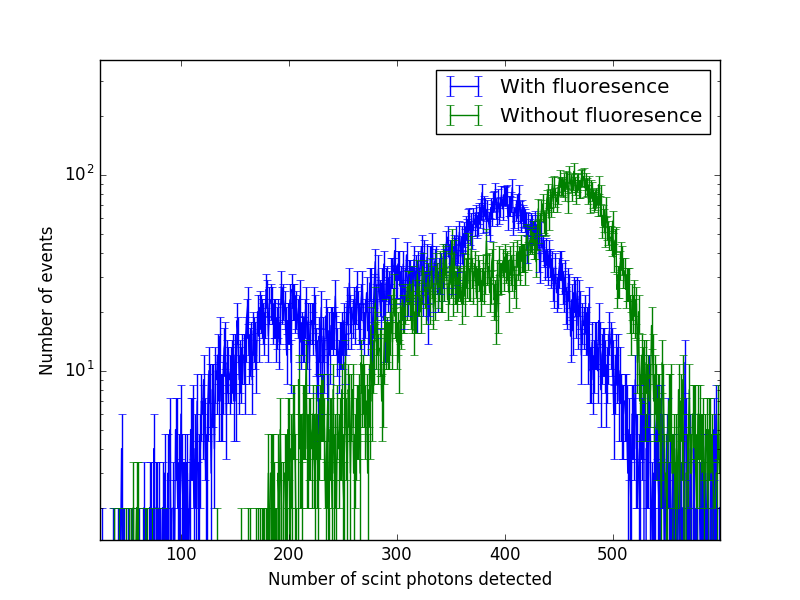
\includegraphics[width=140.0mm]{images/fluovsnofluo.png}
\caption{The obtained energy spectra from simulation with and without x-ray fluoresence being turned on. One can see that, the first peak, which can be seen in the experiments only appear when x-ray fluorescence was turned on.}
\label{fig:fluo}
\end{figure}

\pagebreak

\subsubsection{Calibration of the position dependence}

The main aim of this thesis is to predict what signal the satellite would measure in space. In order to fine tune the parameters of the simulation experimental data was used. The light yield from different parts of the detector is different as scintillation photons have to travel a different distance and they need to be reflected back from the ESR tape that is wrapped around the detector.

\begin{figure}[h!]
\centering
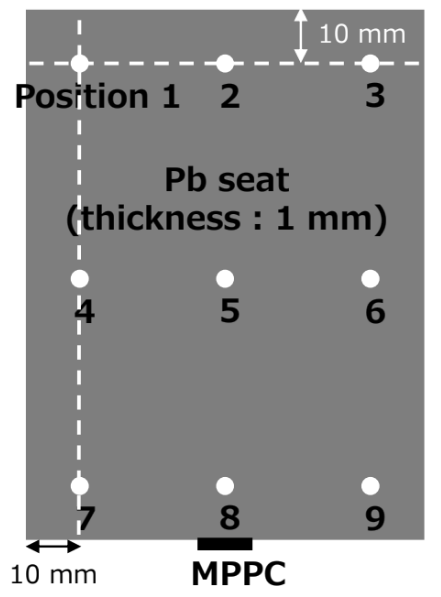
\includegraphics[width=80.0mm]{images/positions.png}
\caption{The positions of irradiation for the investigation of the response of the scintillator}
\end{figure}

A lead sheet was drilled with nine holes to collimate the $\gamma$ source to certain parts of the scintillator. These measurements were carried out by Kento Torigoe at the University of Hiroshima. This configuration with a lead sheet was built up in Geant4 (fig. \ref{fig:sim_setup} and 3.6 million $\gamma$s were simulated at each position. 

\begin{table}[h!]
\begin{center}
\begin{tabular}{ |c|c|c|c|c|c|c|c|c|c| } 
 \hline
  Pos. of source & 1 & 2 & 3 & 4 & 5 & 6 & 7 & 8 & 9 \\ 
  Pos. of main peak & 0.642 & 0.664 & & 70.7 & 0.743 & & 0.598 & &  \\ 
 \hline
\end{tabular}
\label{tab:exp_sim}
\caption{The position dependence of the photon yield measured at the Univeristy of Hiroshima by Kento Torigoe}
\end{center}
\end{table}

The three most relevant parameters of the setup in this case are the scintillation photon yield of the scintillator, the reflection rate of the ESR tape and the self-absorption of the scintillator. The photon yield was fixed to 540 $keV^{-1}$ taken from the data sheet of the scintillator \cite{scinti}. The self-absorption and the reflection rate was increased until the position dependence was the same as in the experiment (table. \ref{tabl:simulated}). 

%ADC / energy calibration from measurement 20170829 illetve az egy chanellel: grb\_status3 

\begin{table}[h!]
\begin{center}
\begin{tabular}{ |c|c|c|c|c|c|c|c|c|c| } 
\hline
Refl:& 0.995 & Abs.:& 50 cm   &  &  &  &  &  &  \\ 
\hline
 Pos. of source & 1 & 2 & 3 & 4 & 5 & 6 & 7 & 8 & 9 \\ 
 Pos. of main peak & 0.4013 & 0.3917 & 0.3981 & 0.4045 & 0.4172 & 0.4140 & 0.2580 & 1 & 0.2739\\ 
 \hline   
\hline
 Refl:& 0.997 & Abs.:& 60 cm   &  &  &  &  &  &  \\ 
 \hline
  Pos. of source & 1 & 2 & 3 & 4 & 5 & 6 & 7 & 8 & 9 \\ 
  Pos. of main peak & 0.4588 & 0.4587 & 0.4697 & 0.4734 & 0.4700 & 0.4737 & 0.3388 & 1 & 0.3365  \\ 
 \hline \hline
Refl:& 0.999 & Abs.:& 80 cm   &  &  &  &  &  &  \\ 
 \hline
  Pos. of source & 1 & 2 & 3 & 4 & 5 & 6 & 7 & 8 & 9 \\ 
  Pos. of main peak &  &  &  &  &  &  &  & 1 &   \\ 
 \hline \hline
Refl:& 0.9996 & Abs.:& 80 cm   &  &  &  &  &  &  \\ 
 \hline
  Pos. of source & 1 & 2 & 3 & 4 & 5 & 6 & 7 & 8 & 9 \\ 
  Pos. of main peak &  &  &  &  &  &  &  & 1 &  \\ 
  \hline
\end{tabular}
 \caption{The position of the Gaussian peak fitted to the 60 keV peak of the Am source for several irradiated positions}
 \label{tabl:simulated}
\end{center}
\end{table}

\subsubsection{Calibration of photon yield}

In the simulation 3.6 million $\gamma$s were simulated. The measurement took 240 s. Therefore the number of photons emitted by the source was $\sim$ 11.0 million. The amplitude of the peaks in the energy spectrum of signal obtained by the MPPC depends mostly on three parameters. The absorption length of the scintillation light in the scintillator, the reflectivity of the surface and the scintillation photon yield of the scintillator. In order to obtain the histogram that we would measure by the MPPC, the histogram obtained by the simulation had to be scaled up both in amplitude and energy. (The introduction of an offset was not needed as the origin point of the histogram obtained in the measurements was shifted to zero energy.)

\begin{figure}[h!]
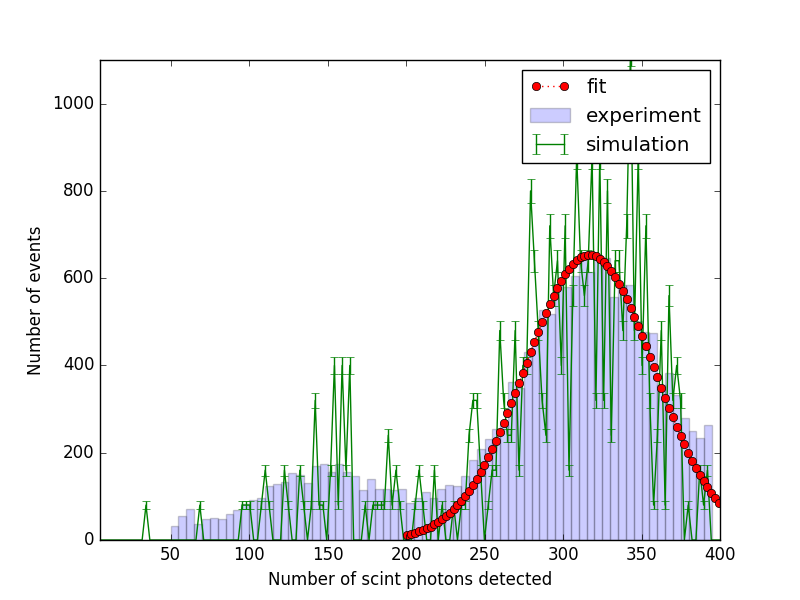
\includegraphics[width=150.0mm]{images/calibration_photon_yield.png}[H!]
\caption{The spectra of 11 million photons taken experimentally (blue histogram) matched up with the results of the simulation (green histogram) and the Gaussian fitted to the simulated data}
\end{figure}

The energy bins had to be scaled up by a factor of 2.4 to match the experimental results. The amplitude had to be scaled up by a factor of 26.2.

\pagebreak

\subsection{Simulation of the signal induced by GRBs in the satellite}

One of the key questions is whether 




\subsection{Simulation of the cosmic background in space}

SPENVIS \cite{spenvis}

"SPENVIS is ESA's SPace ENVironment Information System, a WWW interface to models of the space environment and its effects; including cosmic rays, natural radiation belts, solar energetic particles, plasmas, gases, and "micro-particles"."

\subsubsection{Proton background}

In order to include the resonances in the cross section of the hadron-hadron interactions, additional physics models are needed to be included in the simulation. The signal induced by these resonances might affect the measurement of the protons.


\begin{figure}[htbp]
 \centering % \begin{center}/\end{center} takes some additional vertical space
 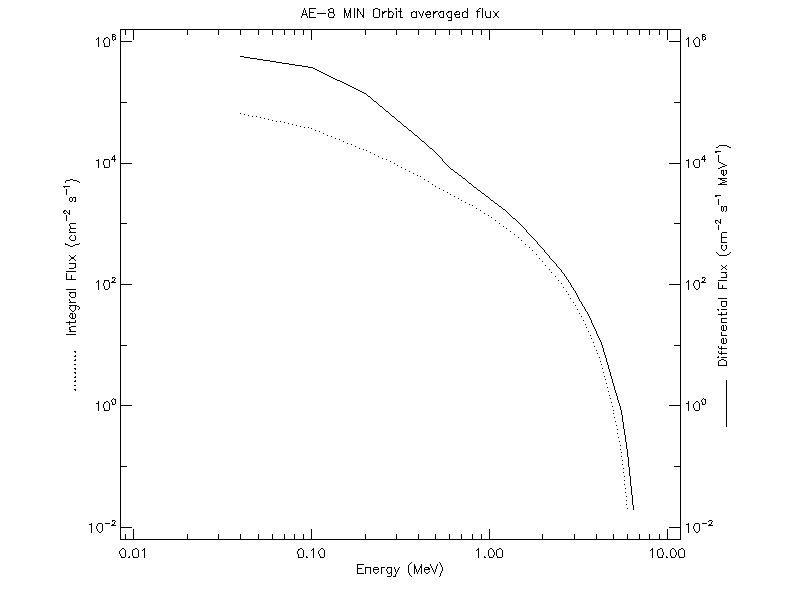
\includegraphics[width=0.45\textwidth,origin=c,angle=0]{images/alt_500km_AE-8_MIN_averaged_spectra.png}
 \qquad
 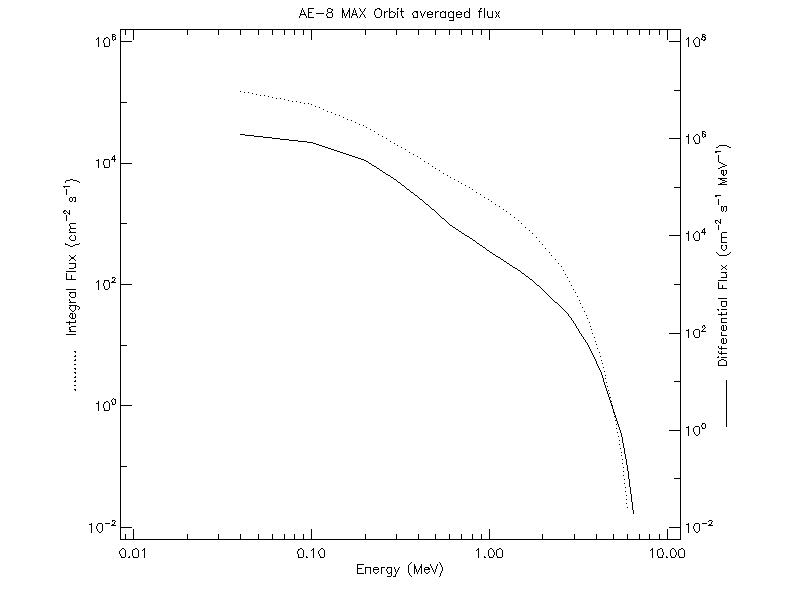
\includegraphics[width=.45\textwidth,origin=c]{images/alt_500km_AE-8_MAX_averaged_spectra.png} 
 % "\includegraphics" from the "graphicx" permits to crop (trim+clip)
 % and rotate (angle) and image (and much more)
 \caption{\label{fig:band500e} The spatially avaraged band function (differential flux for a given energy band, solid line) and the integrated band function (dotted line) of electrons at an altitude of 500 km for solar minimum (left) and solar maximum (right) }
 \end{figure}


Protons
'Apogee: 500.0 km'
'Perigee: 500.0 km'
'Inclination: 89.0 deg'

\subsection{Electron background}

Electrons
'Trapped electron model: AE-8 MIN'
%'Energy','MeV','Energy'
%'IFlux','cm^-2 s^-1','Integral Flux'
%'DFlux','cm^-2 s^-1 MeV^-1','Differential Flux'

\begin{figure}[htbp]
 \centering % \begin{center}/\end{center} takes some additional vertical space
 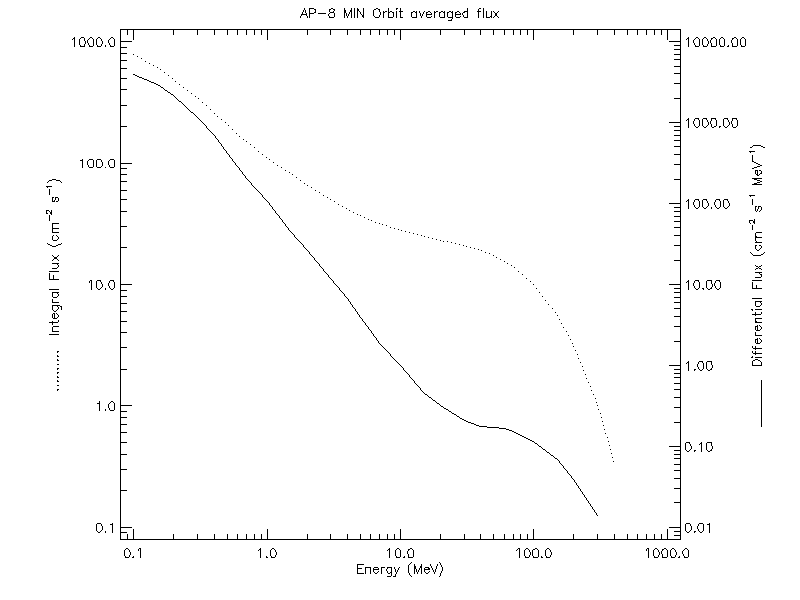
\includegraphics[width=.45\textwidth,origin=c,angle=0]{images/alt_500km_AP-8_MIN_averaged_spectra.png}
 \qquad
 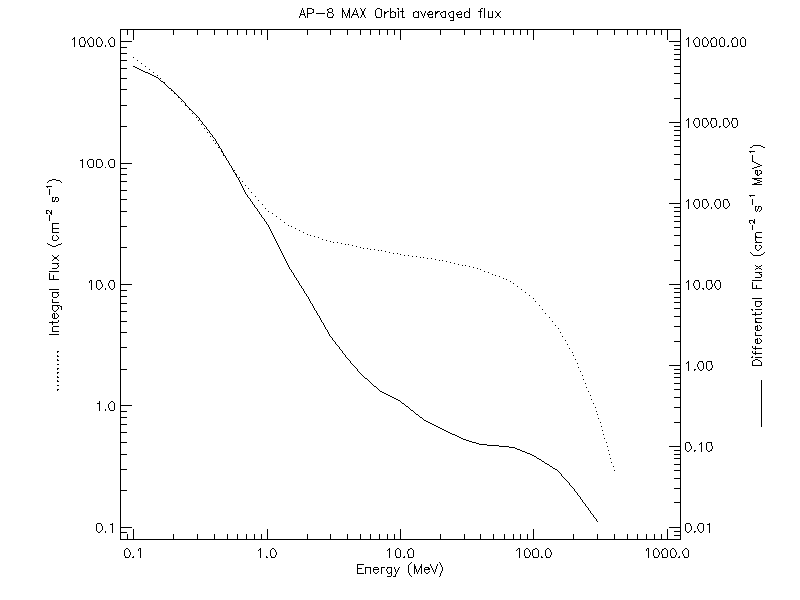
\includegraphics[width=.45\textwidth,origin=c]{images/alt_500km_AP-8_MAX_averaged_spectra.png} 
 % "\includegraphics" from the "graphicx" permits to crop (trim+clip)
 % and rotate (angle) and image (and much more)
 \caption{\label{fig:band500p} The spatially avaraged band function (differential flux for a given energy band, solid line) and the integrated band function (dotted line) of protons at an altitude of 500 km for solar minimum (left) and solar maximum (right) }
 \end{figure}


\begin{figure}[h!]
 \centering % \begin{center}/\end{center} takes some additional vertical space
 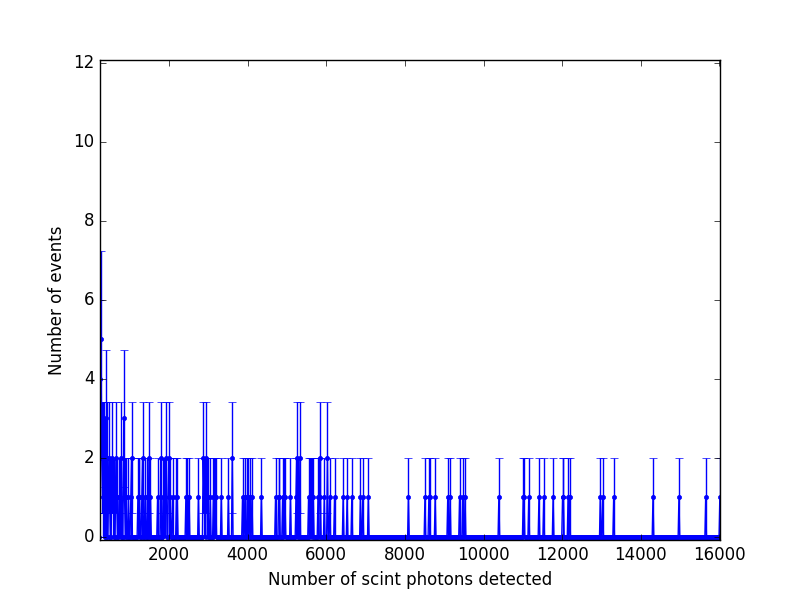
\includegraphics[width=.55\textwidth,origin=c,angle=0]{images/electrons0degspectra.png}
 \qquad
 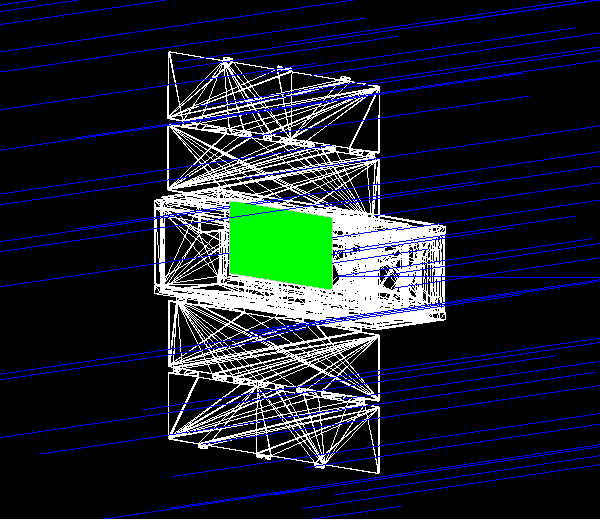
\includegraphics[width=.4\textwidth,origin=c,angle=90]{images/0mac.png} 
 % "\includegraphics" from the "graphicx" permits to crop (trim+clip)
 % and rotate (angle) and image (and much more)
 \caption{\label{fig:i} The spectrum measured when the electrons were shot perpendicular to the scintillator (called angle of 0 $^{\circ}$)}
 \end{figure}

\begin{figure}[h!]
 \centering % \begin{center}/\end{center} takes some additional vertical space
 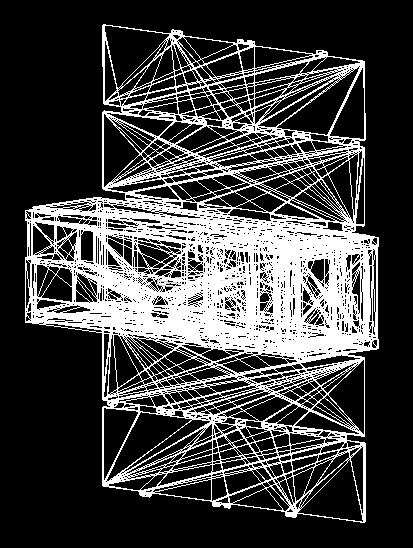
\includegraphics[width=.3\textwidth,origin=c,angle=0]{images/satellite.png}
 \qquad
 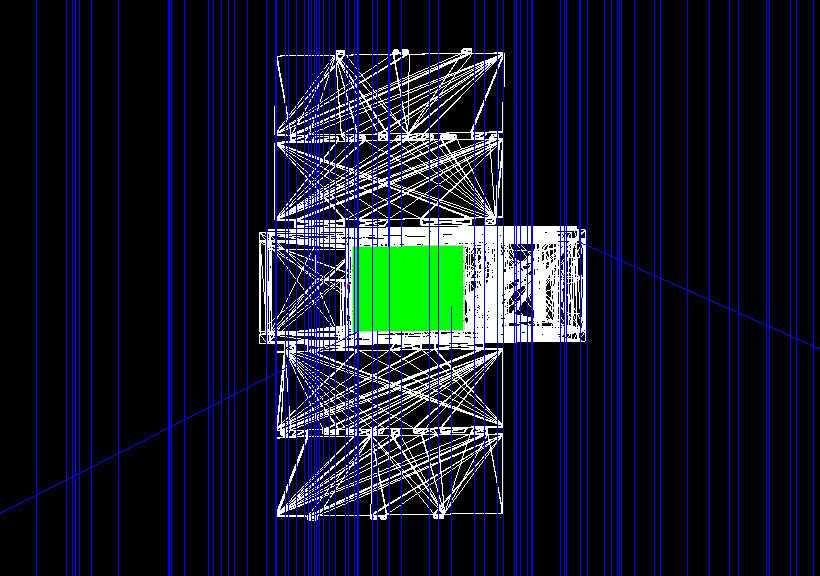
\includegraphics[width=.5\textwidth,origin=c,angle=90]{images/8mac.png} 
 % "\includegraphics" from the "graphicx" permits to crop (trim+clip)
 % and rotate (angle) and image (and much more)
 \caption{\label{fig:i} The CAD model of the satellite (on the right) and the view of the imported model in Geant (on the left)}
 \end{figure}

\begin{figure}[h!]
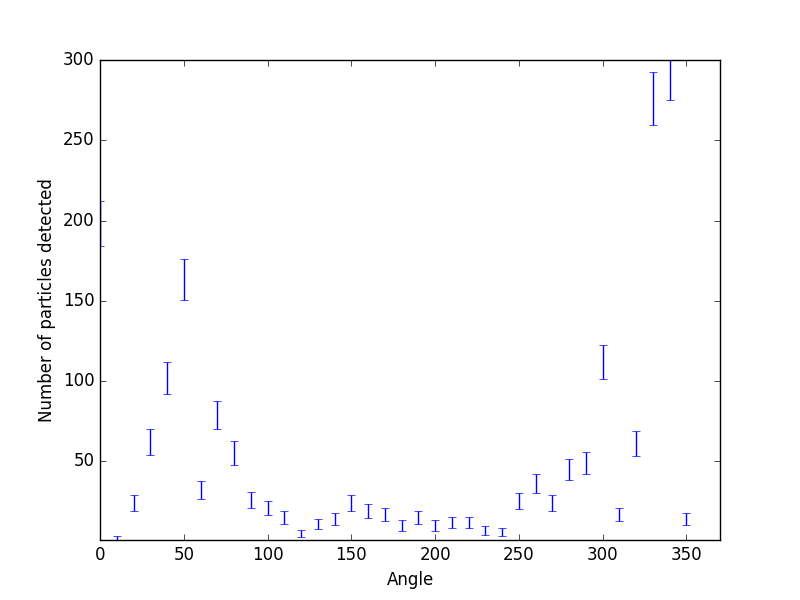
\includegraphics[width=150.0mm]{images/electronabsorption.png}[H!]
\caption{The ammount of electrons detected from 100.000 shoot in the simulation}
\end{figure}

\subsubsection{$\gamma$ background}

\pagebreak

Put 4 spectra here from the 4 direction to the satellite. Quantify the detected photons by summing up all entries. Where should be the treshold?

CHange the mass of the payload!

\pagebreak

\section{Conclusion}

In order to simulate how the Camelot CubeSat would interact with the cosmic background and how sensitive it would be to GRBs that it is designed to investigate a Geant4 simulation was built.

As the first step, the experimental setup that was used to test the CsI(Tl) scintillator -- the particle detector of the satellite -- was implemented in Geant4. The optical parameters of the simulation were fine tuned by comparing the light yield of the MPPCs that was used to read out the scintillator. After the calibration, the results of the simulation was capable of predicting the signal that would be measured in space.

Secondly, the complex CAD model of the satellite --consisting of 7 modules, each with a give avarage material composition-- was exported to Geant4. The scintillator and its read out was placed on the side of the satellite.

Thirdly, the $\gamma$ absorption of the satellite was invastigated. Parallel $\gamma$-rays with a flux and energy distribution of GRB 9900123 (fig. \ref{fig:grb_band}) was simulated. 36 positions were investigated by varying the incident angle of the $\gamma$s around the major axis of the satellite.

The results show...


Fourthly, the effect of cosmic radiation was invastigated by utilizing the energy spectra of cosmic protons and electrons at the altitude of 500km. The satellite was radiated by these particles in Geant4 in the same positions that were used for the $\gamma$-rays of GRB 9900123. The induced signal of these particles was determined. This needs to be minimalized as it "competes" with the signal of gamma particles from GRBs.


\pagebreak

\section{Acknowledgment}

Gabor Galg\'oczi would like to thank Bal\'azs \'Ujv\'ari for the fruitful discussions they had on Geant4 simulations. Useful comments on detectors made Dezs\"o Varga's advices on detectors were highly appreciated. András Pál made vital comments on the description of the electronics. Last but not least the author would like to thank Norbert Werner for the continued contributions to this work.

\pagebreak

\addcontentsline{toc}{section}{References}
\begin{thebibliography}{99}
\interlinepenalty=10000

\bibitem{grb1} Mészáros P., 2006, Reports on Progress in Physics, 69, 2259
%https://link.springer.com/content/pdf/10.1007/s11214-017-0366-4.pdf

\bibitem{grb2} Vedrenne G., \& Atteia J.-L., 2009, Gamma-Ray Bursts: The brightest explosions in the Universe,
Springer Praxis Books in Astronomy and Planetary Sciences, Published in association with Praxis
Publishing, UK
%https://link.springer.com/content/pdf/10.1007/s11214-017-0366-4.pdf

\bibitem{grb3} Kouveliotou C., Wijers R. A. M. J., \& Woosley S., 2012, Gamma-ray Bursts, Cambridge, UK:
Cambridge University Press
%https://link.springer.com/content/pdf/10.1007/s11214-017-0366-4.pdf

\bibitem{grb4} Gehrels N., \& Mészáros P. 2012, Science, 337, 932
%https://link.springer.com/content/pdf/10.1007/s11214-017-0366-4.pdf

\bibitem{grb5} Klebesadel R. W., Strong I. B., \& Olson R. A. 1973, The Astrophysical Journal, 182, L85

\bibitem{grb6} Kouveliotou C., Meegan C. A., Fishman G. J., et al. 1993, The Astrophysical Journal Letters, 413, L101

\bibitem{grb7} Balázs L. G., Bagoly Z., Horváth I., et al. 2003, Astronomy and Astrophysics, 401, 129

\bibitem{grb8} Mészáros A., Bagoly Z., Balázs L. G., \& Horváth I. 2006, Astronomy and Astrophysics, 455, 785

\bibitem{grb9} Berger E. 2014, Annual Review of Astronomy and Astrophysics, 52, 43

\bibitem{grb10} Rees M. J., \& Meszaros P. 1994, The Astrophysical Journal, 430, L93

\bibitem{grb11} van Paradijs J., Groot P. J., Galama T., et al. 1997, Nature, 386, 686

\bibitem{grb12} Paczynski B. 1986, The Astrophysical Journal, 308, L43

\bibitem{grb14} Fruchter A. S., Levan A. J., Strolger L., et al. 2006, Nature, 441, 463

\bibitem{gravwave} https://arxiv.org/abs/1710.05834

\bibitem{grb17} Abbott B. P., Abbott R., Abbott T. D., et al. 2017, Physical Review Letters, 119, 161101

\bibitem{grb18} Tanvir N. R., Levan A. J., Fruchter A. S., et al. 2013, Nature, 500, 547

\bibitem{grb19} Zhang, B. 2011, Comptes Rendus Physique, 12, 206

\bibitem{grb20} Toma, K., Yoon, S.-C., \& Bromm, V. 2016, Space Science Reviews, 202, 159

\bibitem{grb21} Goldstein A., et al., 2017, The Astrophysical Journal Letters, 848, L14

\bibitem{grb22} Savchenko V., et al., 2017, The Astrophysical Journal Letters, 848, L15

\bibitem{grb23} Troja E., et al., 2017, Naure, 551, 71

\bibitem{grb24} Evans P. A., Cenko S. B., Kennea J. A., et al. 2017, Science, 358, 1565

\bibitem{grb25} Loeb A., 2016, The Astrophysical Journal Letters, 819, L21

\bibitem{grb26} KAGRA Collaboration, Akutsu T., Ando M., et al. 2017, arXiv:1710.04823

\bibitem{grb27} Cavallari E., \& Frontera F. 2017, Space Science Reviews, 212, 429
 
\bibitem{grb28} Atwood, W. B., \& GLAST Collaboration 1994, Nuclear Instruments and Methods in Physics Research
A, 342, 302

\bibitem{grb30} Cavallari E., \& Frontera F. 2017, Space Science Reviews, 212, 429

\bibitem{grb31} Barthelmy S. D., Barbier L. M., Cummings J. R., et al. 2005, Space Science Reviews, 120, 143

\bibitem{grb32} Winkler C., Courvoisier T. J.-L., Di Cocco G., et al. 2003, Astronomy and Astrophysics, 411, L1

\bibitem{grb34} Tavani M., Barbiellini G., Argan A., et al. 2009, Astronomy and Astrophysics, 502, 995

\bibitem{grb35} Yamaoka K., Yoshida A., Nonaka Y. 2011, 32nd International Cosmic Ray Conference, 9, 111

\bibitem{grb36} Serino M., Sakamoto T., Kawai N., et al. 2014, Publications of the Astronomical Society of Japan, 66,
87

\bibitem{grb37} Produit N., Barao F., Deluit S., et al. 2005, Nuclear Instruments and Methods in Physics Research A,
550, 616

\bibitem{grb38} Sadovnichii V. A., Panasyuk M. I., Amelyushkin A. M., et al. 2017, Space Science Reviews, 212, 1705

\bibitem{grb39} Li T., Xiong S., Zhang S., et al. 2018, Science China Physics, Mechanics, and Astronomy, 61, 31011

\bibitem{grb40} Navalgund K. H., Suryanarayana Sarma K., Gaurav P. K., Nagesh G., \& Annadurai M. 2017, Journal of Astrophysics and Astronomy, 38, 34

\bibitem{grb41} Lin R. P., Dennis B. R., Hurford G. J., et al. 2002, Solar Physics, 210, 3

\bibitem{grb42} Hurley K., Mitrofanov I. G., Golovin D., et al. 2013, EAS Publications Series, 61, 459 

\bibitem{grb43} Lipunov V., Kornilov V., Gorbovskoy E., et al. 2016, Revista Mexicana de Astronomia y Astrofisica
Conference Series, 48, 42

\bibitem{grb44} Castro-Tirado A. J., Soldán J., Bernas M., et al. 1999, Astronomy and Astrophysics Supplement, 138, 583

\bibitem{grb45} Akerlof C. W., Kehoe R. L., McKay T. A., et al. 2003, Publications of the Astronomical Society of the Pacific, 115, 132

\bibitem{grb46} Majcher A., Batsch T., Castro-Tirado A. J., et al. 2015, Proceedings of SPIE, 9662, 966219

\bibitem{grb_spectra} Gamma-Ray Bursts and Fast Transients
Multi-wavelength Observations and Multi-messenger Signals,\\
R. Willingale, P. Mészáros
%https://link.springer.com/content/pdf/10.1007/s11214-017-0366-4.pdf

\bibitem{geant1} Nuclear Instruments and Methods in Physics Research A 506 (2003) 250-303

\bibitem{geant2} IEEE Transactions on Nuclear Science 53 No. 1 (2006) 270-278

\bibitem{geant3} Nuclear Instruments and Methods in Physics Research A 835 (2016) 186-225

\bibitem{cadmesh} Poole, C. M. and Cornelius, I. and Trapp, J. V. and Langton, C. M., A CAD Interface for GEANT4, Australasian Physical \& Engineering Science in Medicine, 2012

\bibitem{assimp} http://www.assimp.org/

\bibitem{tetgen} Hang Si. 2015. "TetGen, a Delaunay-Based Quality Tetrahedral Mesh Generator". ACM Trans. on Mathematical Software. 41 (2), Article 11 (February 2015), 36 pages

\bibitem{scinti} http://www.amcrys.com/pdf/4279\_.pdf

\bibitem{qe} http://www.hamamatsu.com/resources/pdf/ssd/s13360\_series\_kapd1052e.pdf

\bibitem{esr} http://multimedia.3m.com/mws/media/466120O/esr.pdf
 
\bibitem{spenvis} https://www.spenvis.oma.be/

\end{thebibliography}

\pagebreak

\listoffigures

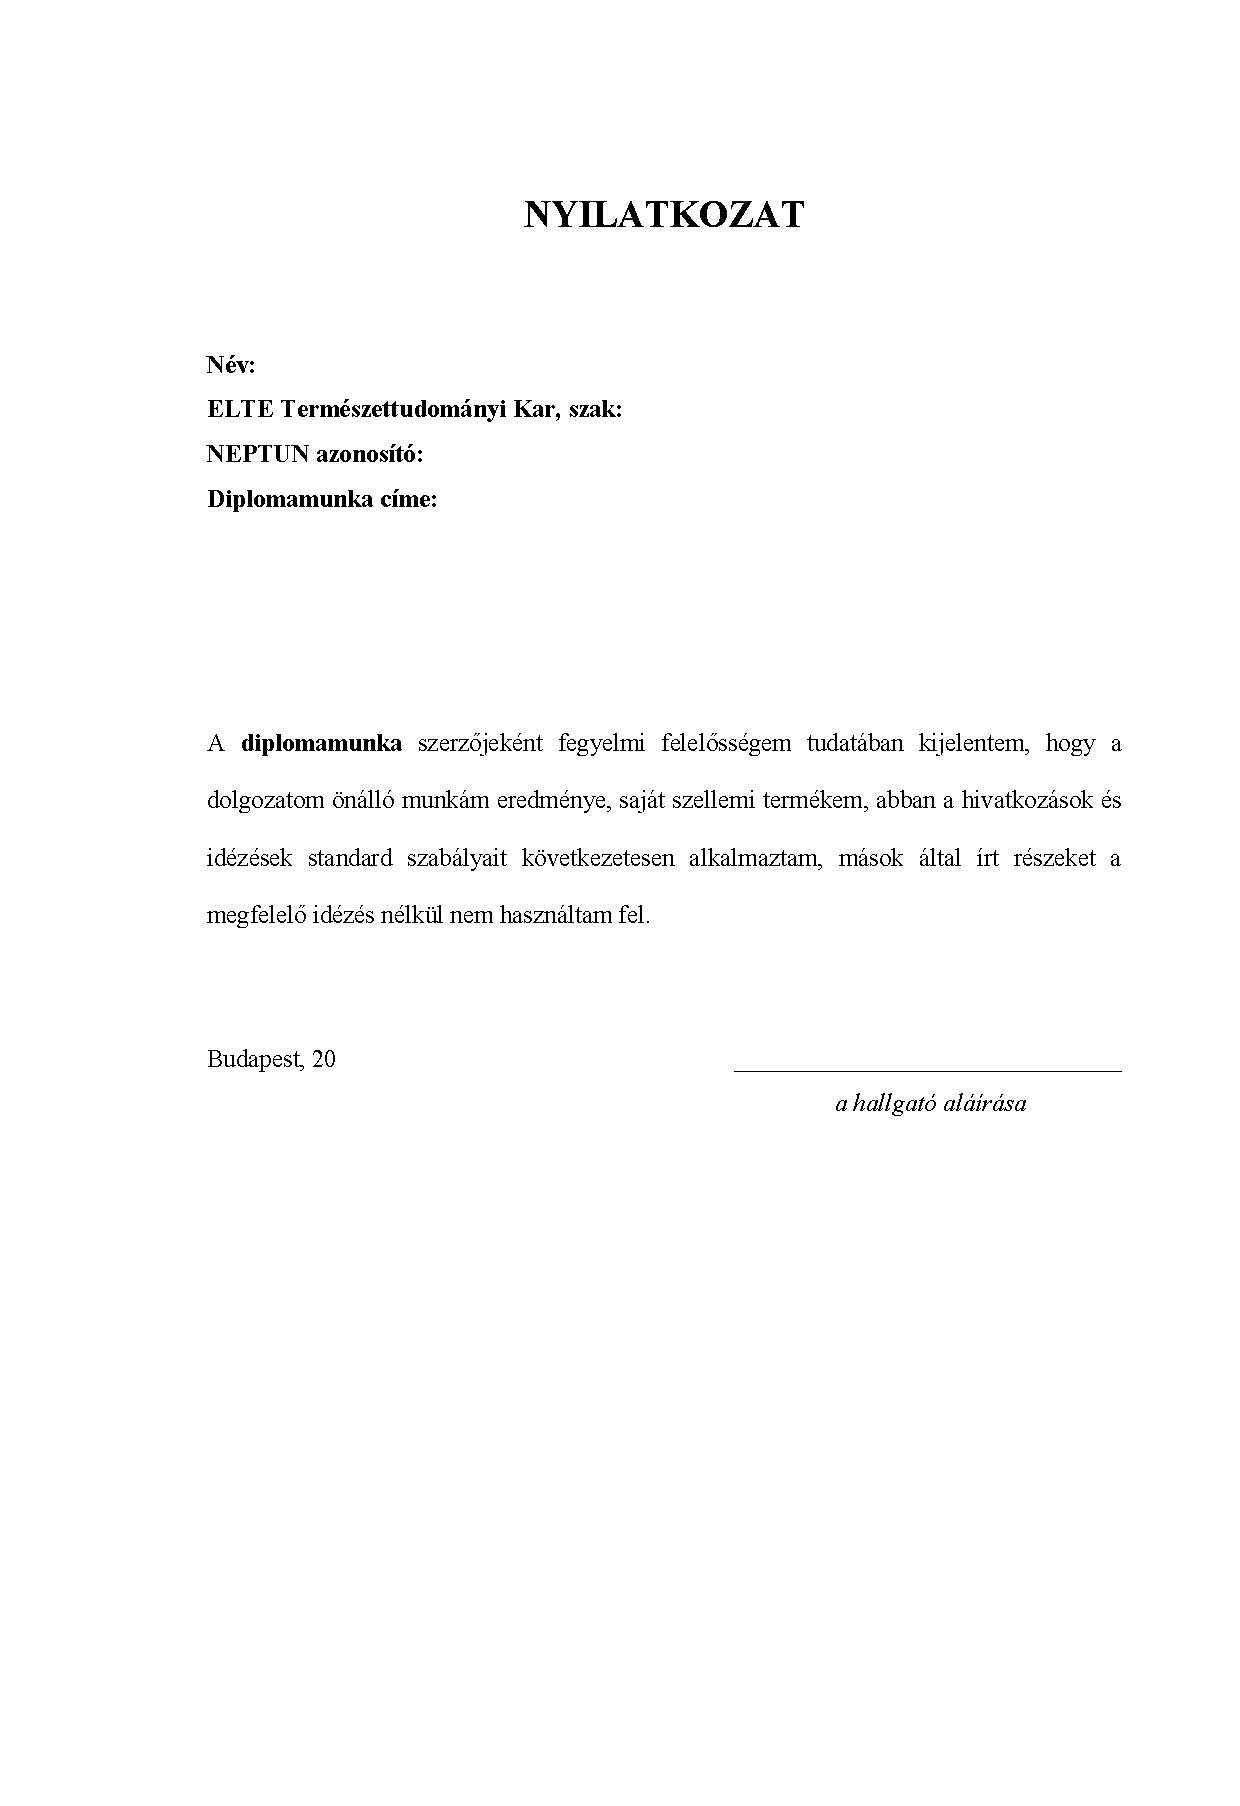
\includepdf[pages=-,pagecommand={},width=\textwidth]{images/nyilatkozat.pdf}



\end{document}

\begin{figure}[h!]
\centerline{
\includegraphics[width=260pt,angle=0]{images/let_setup.png}}
\caption{Az általam használt OTPC a gázrendszerével, illetve a kiolvasórendszerével együtt}
\end{figure}

Sötét anyag kutatásra jó beveztő:
https://arxiv.org/pdf/1510.02170.pdf
Nuclear physics:
https://indico.fnal.gov/conferenceDisplay.py/abstractBook?confId=8976

%%%%%%%%%%%%%%%
Alkalmazások


M. Pomorski, M. Pfutzner
M. Pomorski et al. Phys. Rev. C 90, 014311 (2014)

Micromegas-os kiolvasás J. B. R. Battat, Nucl. Instr. Meth. A 755(2014)6.

[grid???] U. Titt, V. Dagendorf et al., (Nucl. Instr. Meth. A 477 (2002) 536:	 
grids, pure TEA at low pressure, (electron counting / nano-dosimetry)

%%%%%%%%%%%%%%

Performance of an optical readout GEM-based TPC, L.M.S. Margato a...

optikai úton kiolvasott tpc-k: florian e-mailjéből

LET TPC

radon és polónium energiáira cikkek